\RequirePackage{flashmovie}
\documentclass[hide notes,intlimits]{beamer}


\mode<presentation>
{
  \usetheme{UAFshade}
  \setbeamercovered{transparent}
}

% load packages
\usepackage{multimedia}
\usepackage{animate}
\usepackage[english]{babel}
\usepackage[latin1]{inputenc}
\usepackage[T1]{fontenc}
\usepackage{lmodern}
\usepackage[multidot]{grffile}
\usepackage[amssymb]{SIunits}
% \usepackage{flashmovie}
\usepackage{tikz}
\usetikzlibrary{shapes,arrows,shadows, calc}

% \usepackage{pgfpages}
% \setbeamertemplate{note page}[plain]
% \setbeameroption{show notes on second screen=right}


\definecolor{dark red}{HTML}{E41A1C}
\definecolor{dark green}{HTML}{4DAF4A}
\definecolor{dark violet}{HTML}{984EA3}
\definecolor{dark blue}{HTML}{084594}
\definecolor{dark orange}{HTML}{FF7F00}
\definecolor{white}{HTML}{FFFFFF}
\definecolor{light blue}{HTML}{377EB8}
\definecolor{light red}{HTML}{FB9A99}
\definecolor{light violet}{HTML}{CAB2D6}

\definecolor{uaf red}{HTML}{E41A1C}
\definecolor{uaf blue}{HTML}{377EB8}
\definecolor{uaf green}{HTML}{4DAF4A}
\definecolor{uaf violet}{HTML}{984EA3}
\definecolor{uaf orange}{HTML}{FF7F00}
\setbeamercolor{boxed}{fg=black,bg=uaf yellow}


% Define block styles
\tikzstyle{initialization} = [ellipse, draw, 
    text badly centered, draw=dark violet,
        % The filling: 
        top color=white, 
        bottom color=dark violet]
\tikzstyle{initialization faded} = [ellipse, draw, 
    text badly centered, draw=dark violet!50,
        % The filling: 
        top color=white, 
        bottom color=dark violet!25]
\tikzstyle{hindcast} = [ellipse, draw,
    text badly centered, rounded corners,draw=dark orange,
        % The filling: 
        top color=white, 
        bottom color=dark orange]
\tikzstyle{hindcast faded} = [ellipse, draw,
    text badly centered, rounded corners,draw=dark orange!50,
        % The filling: 
        top color=white, 
        bottom color=dark orange!25]
\tikzstyle{forecast} = [ellipse, draw,
    text badly centered, rounded corners,draw=dark blue,
        % The filling: 
        top color=white, 
        bottom color=dark blue]
\tikzstyle{forecast faded} = [ellipse, draw,
    text badly centered, rounded corners,draw=dark blue!50,
        % The filling: 
        top color=white, 
        bottom color=dark blue!50]
\tikzstyle{arrow line} = [draw, -latex']
\tikzstyle{line} = [draw]



\graphicspath{{figures/}}

\setbeamerfont{caption}{size=\scriptsize}

% code adapted from http://tex.stackexchange.com/a/11483/3954

% some parameters for customization
\def\shadowshift{3pt,-3pt}
\def\shadowradius{6pt}

\colorlet{innercolor}{black!60}
\colorlet{outercolor}{gray!05}

% this draws a shadow under a rectangle node
\newcommand\drawshadow[1]{
    \begin{pgfonlayer}{shadow}
        \shade[outercolor,inner color=innercolor,outer color=outercolor] ($(#1.south west)+(\shadowshift)+(\shadowradius/2,\shadowradius/2)$) circle (\shadowradius);
        \shade[outercolor,inner color=innercolor,outer color=outercolor] ($(#1.north west)+(\shadowshift)+(\shadowradius/2,-\shadowradius/2)$) circle (\shadowradius);
        \shade[outercolor,inner color=innercolor,outer color=outercolor] ($(#1.south east)+(\shadowshift)+(-\shadowradius/2,\shadowradius/2)$) circle (\shadowradius);
        \shade[outercolor,inner color=innercolor,outer color=outercolor] ($(#1.north east)+(\shadowshift)+(-\shadowradius/2,-\shadowradius/2)$) circle (\shadowradius);
        \shade[top color=innercolor,bottom color=outercolor] ($(#1.south west)+(\shadowshift)+(\shadowradius/2,-\shadowradius/2)$) rectangle ($(#1.south east)+(\shadowshift)+(-\shadowradius/2,\shadowradius/2)$);
        \shade[left color=innercolor,right color=outercolor] ($(#1.south east)+(\shadowshift)+(-\shadowradius/2,\shadowradius/2)$) rectangle ($(#1.north east)+(\shadowshift)+(\shadowradius/2,-\shadowradius/2)$);
        \shade[bottom color=innercolor,top color=outercolor] ($(#1.north west)+(\shadowshift)+(\shadowradius/2,-\shadowradius/2)$) rectangle ($(#1.north east)+(\shadowshift)+(-\shadowradius/2,\shadowradius/2)$);
        \shade[outercolor,right color=innercolor,left color=outercolor] ($(#1.south west)+(\shadowshift)+(-\shadowradius/2,\shadowradius/2)$) rectangle ($(#1.north west)+(\shadowshift)+(\shadowradius/2,-\shadowradius/2)$);
        \filldraw ($(#1.south west)+(\shadowshift)+(\shadowradius/2,\shadowradius/2)$) rectangle ($(#1.north east)+(\shadowshift)-(\shadowradius/2,\shadowradius/2)$);
    \end{pgfonlayer}
}

% create a shadow layer, so that we don't need to worry about overdrawing other things
\pgfdeclarelayer{shadow} 
\pgfsetlayers{shadow,main}

\newsavebox\mybox
\newlength\mylen

\newcommand\shadowimage[2][]{%
\setbox0=\hbox{\includegraphics[#1]{#2}}
\setlength\mylen{\wd0}
\ifnum\mylen<\ht0
\setlength\mylen{\ht0}
\fi
\divide \mylen by 120
\def\shadowshift{\mylen,-\mylen}
\def\shadowradius{\the\dimexpr\mylen+\mylen+\mylen\relax}
\begin{tikzpicture}
\node[anchor=south west,inner sep=0] (image) at (0,0) {\includegraphics[#1]{#2}};
\drawshadow{image}
\end{tikzpicture}}

\newcommand\shadowimagec[3][]{%
\setbox0=\hbox{\includegraphics<#1>[#2]{#3}}
\setlength\mylen{\wd0}
\ifnum\mylen<\ht0
\setlength\mylen{\ht0}
\fi
\divide \mylen by 120
\def\shadowshift{\mylen,-\mylen}
\def\shadowradius{\the\dimexpr\mylen+\mylen+\mylen\relax}
\begin{tikzpicture}
\node[anchor=south west,inner sep=0] (image) at (0,0) {\includegraphics<#1>[#2]{#3}};
\drawshadow{image}
\end{tikzpicture}}


\newenvironment{transbox}[1][]{%
\begin{tikzpicture}
\node[drop shadow,rounded corners,text width=\textwidth,fill=white, fill opacity=#1,text opacity=1] \bgroup
}{
\egroup;\end{tikzpicture}} 

\newenvironment{transbox-tight}{%
\begin{tikzpicture}
\node[drop shadow,rounded corners,fill=uaf yellow, fill opacity=0.75,text opacity=1] \bgroup
}{
\egroup;\end{tikzpicture}} 


% title page
\title[] % (optional, use only with long paper titles)
{Glaciers: The Biggest Losers}



\author[Aschwanden] % (optional, use only with lots of authors)
{Andy Aschwanden}
% - Give the names in the same order as the appear in the paper.
% - Use the \inst{?} command only if the authors have different
%   affiliation.

\institute[Geophysical Institute] % (optional, but mostly needed)
{}
% - Use the \inst command only if there are several affiliations.
% - Keep it simple, no one is interested in your street address.


\date{}

\begin{document}

% define what is shown at the beginning of each section
\AtBeginSection[]
{
  \begin{frame}<handout:0>
    \frametitle{Outline}
   \tableofcontents[currentsection,subsectionstyle=hide/hide/hide]
  \end{frame}
}

% define what is shown at the beginning of each subsection
\AtBeginSubsection[]
{
 \begin{frame}<beamer>
  \frametitle{Outline}
   \tableofcontents[currentsection,currentsubsection]
 \end{frame}
}


\setbeamertemplate{background canvas}
  {
     \tikz{\node[inner sep=0pt,opacity=1.] {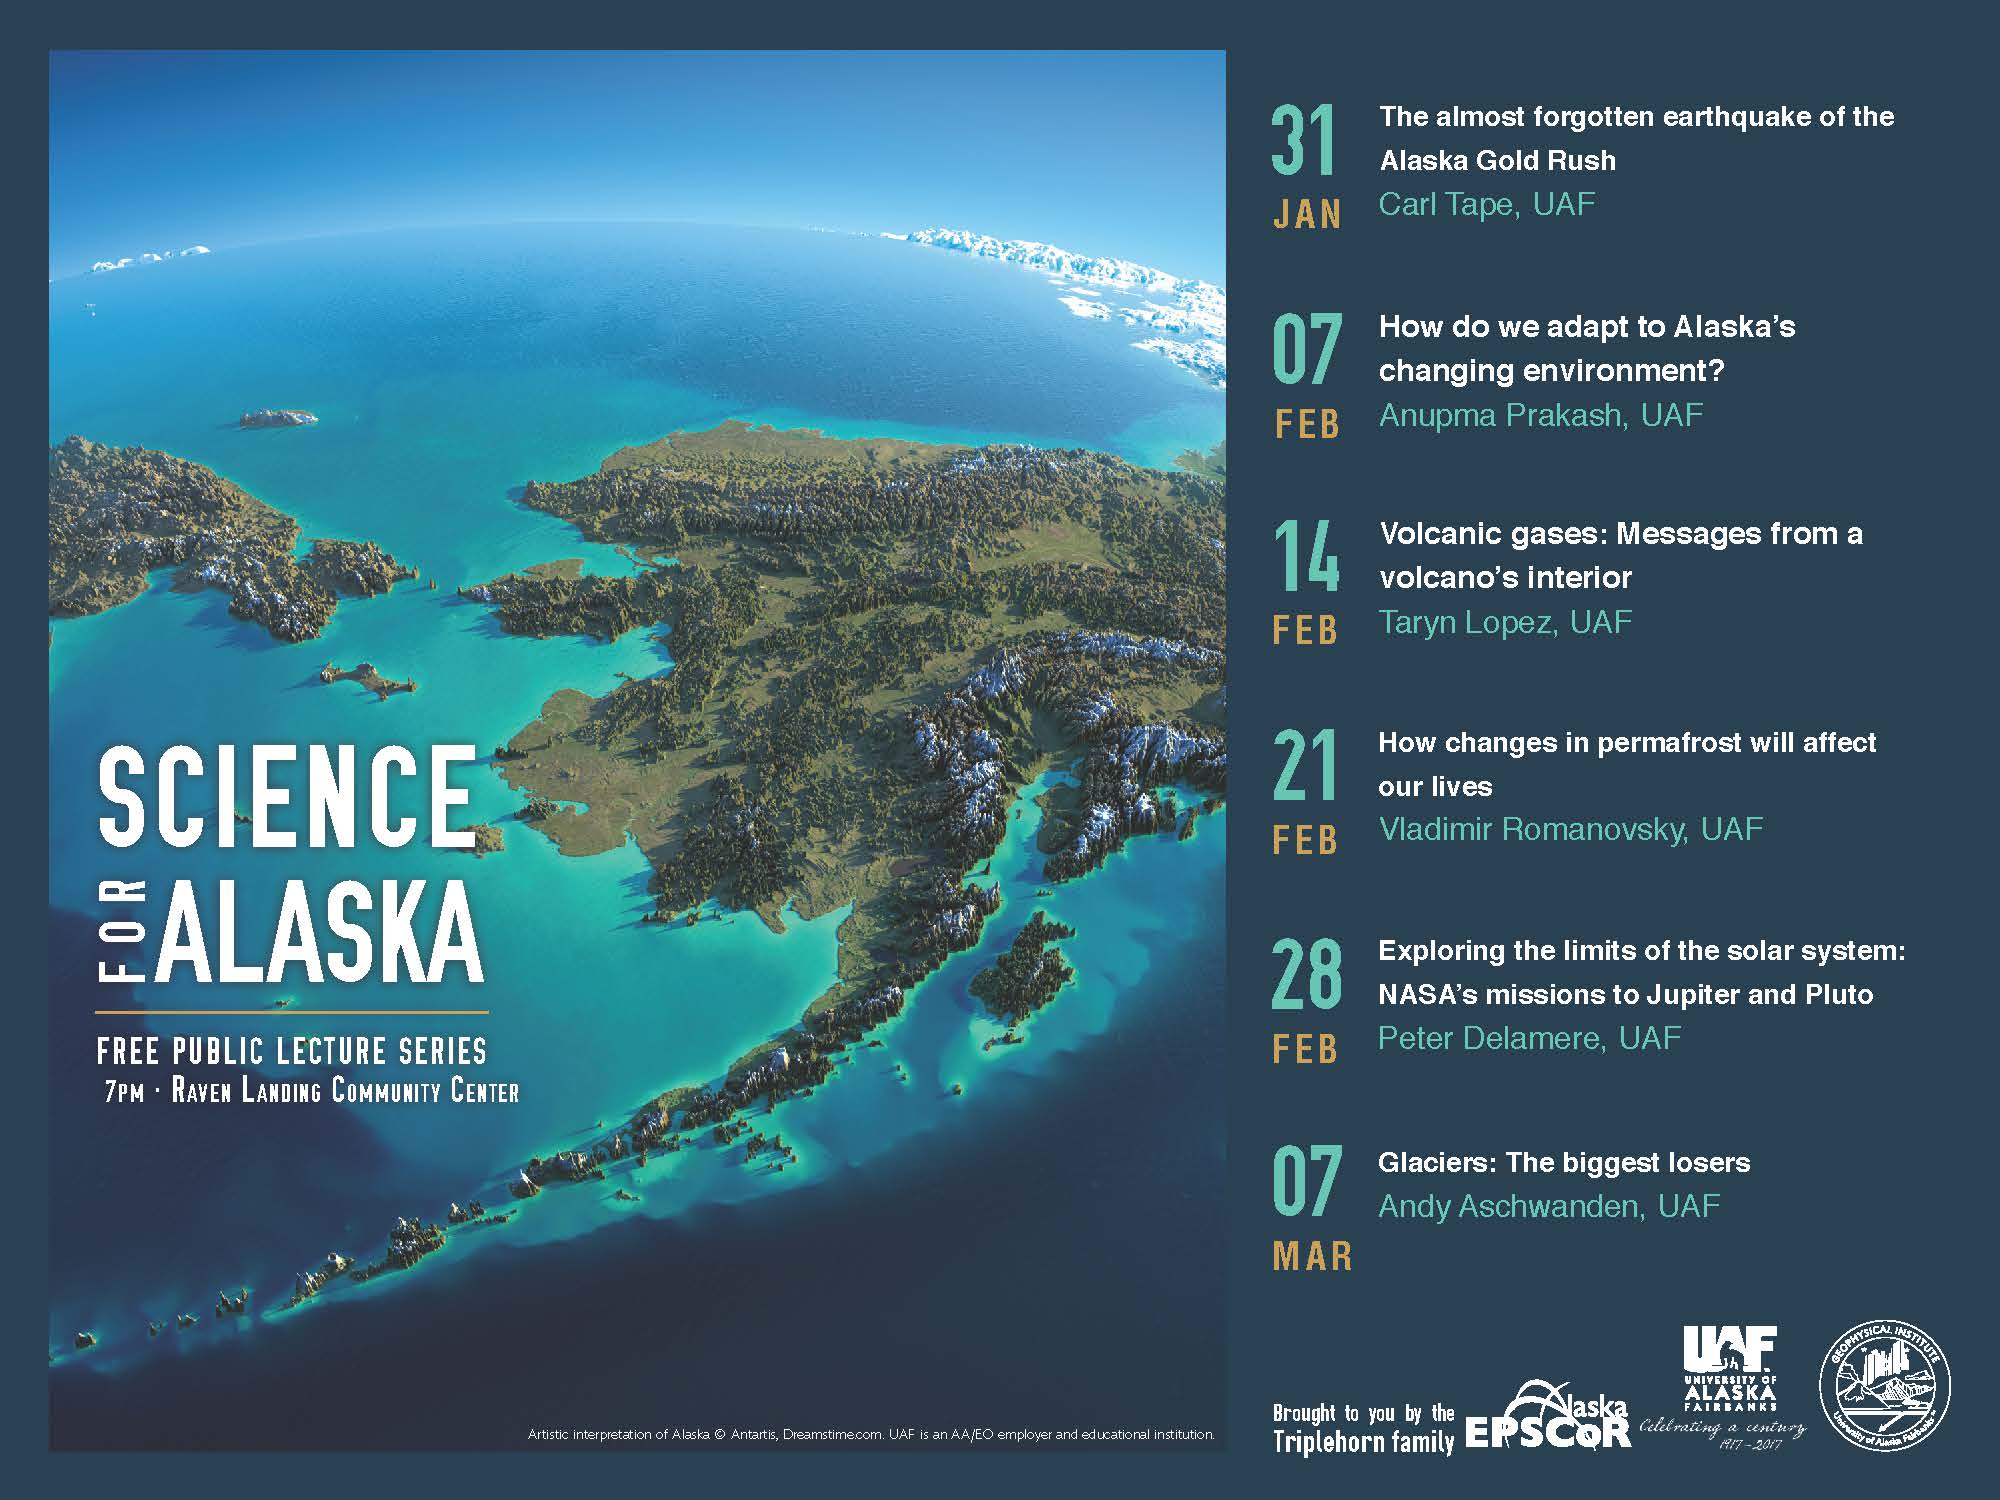
\includegraphics[width=\paperwidth]{SFALS_2017}};}
}

\begin{frame}[plain]
\end{frame}

\setbeamertemplate{background canvas}
  {
     \tikz{\node[inner sep=0pt,opacity=1.] {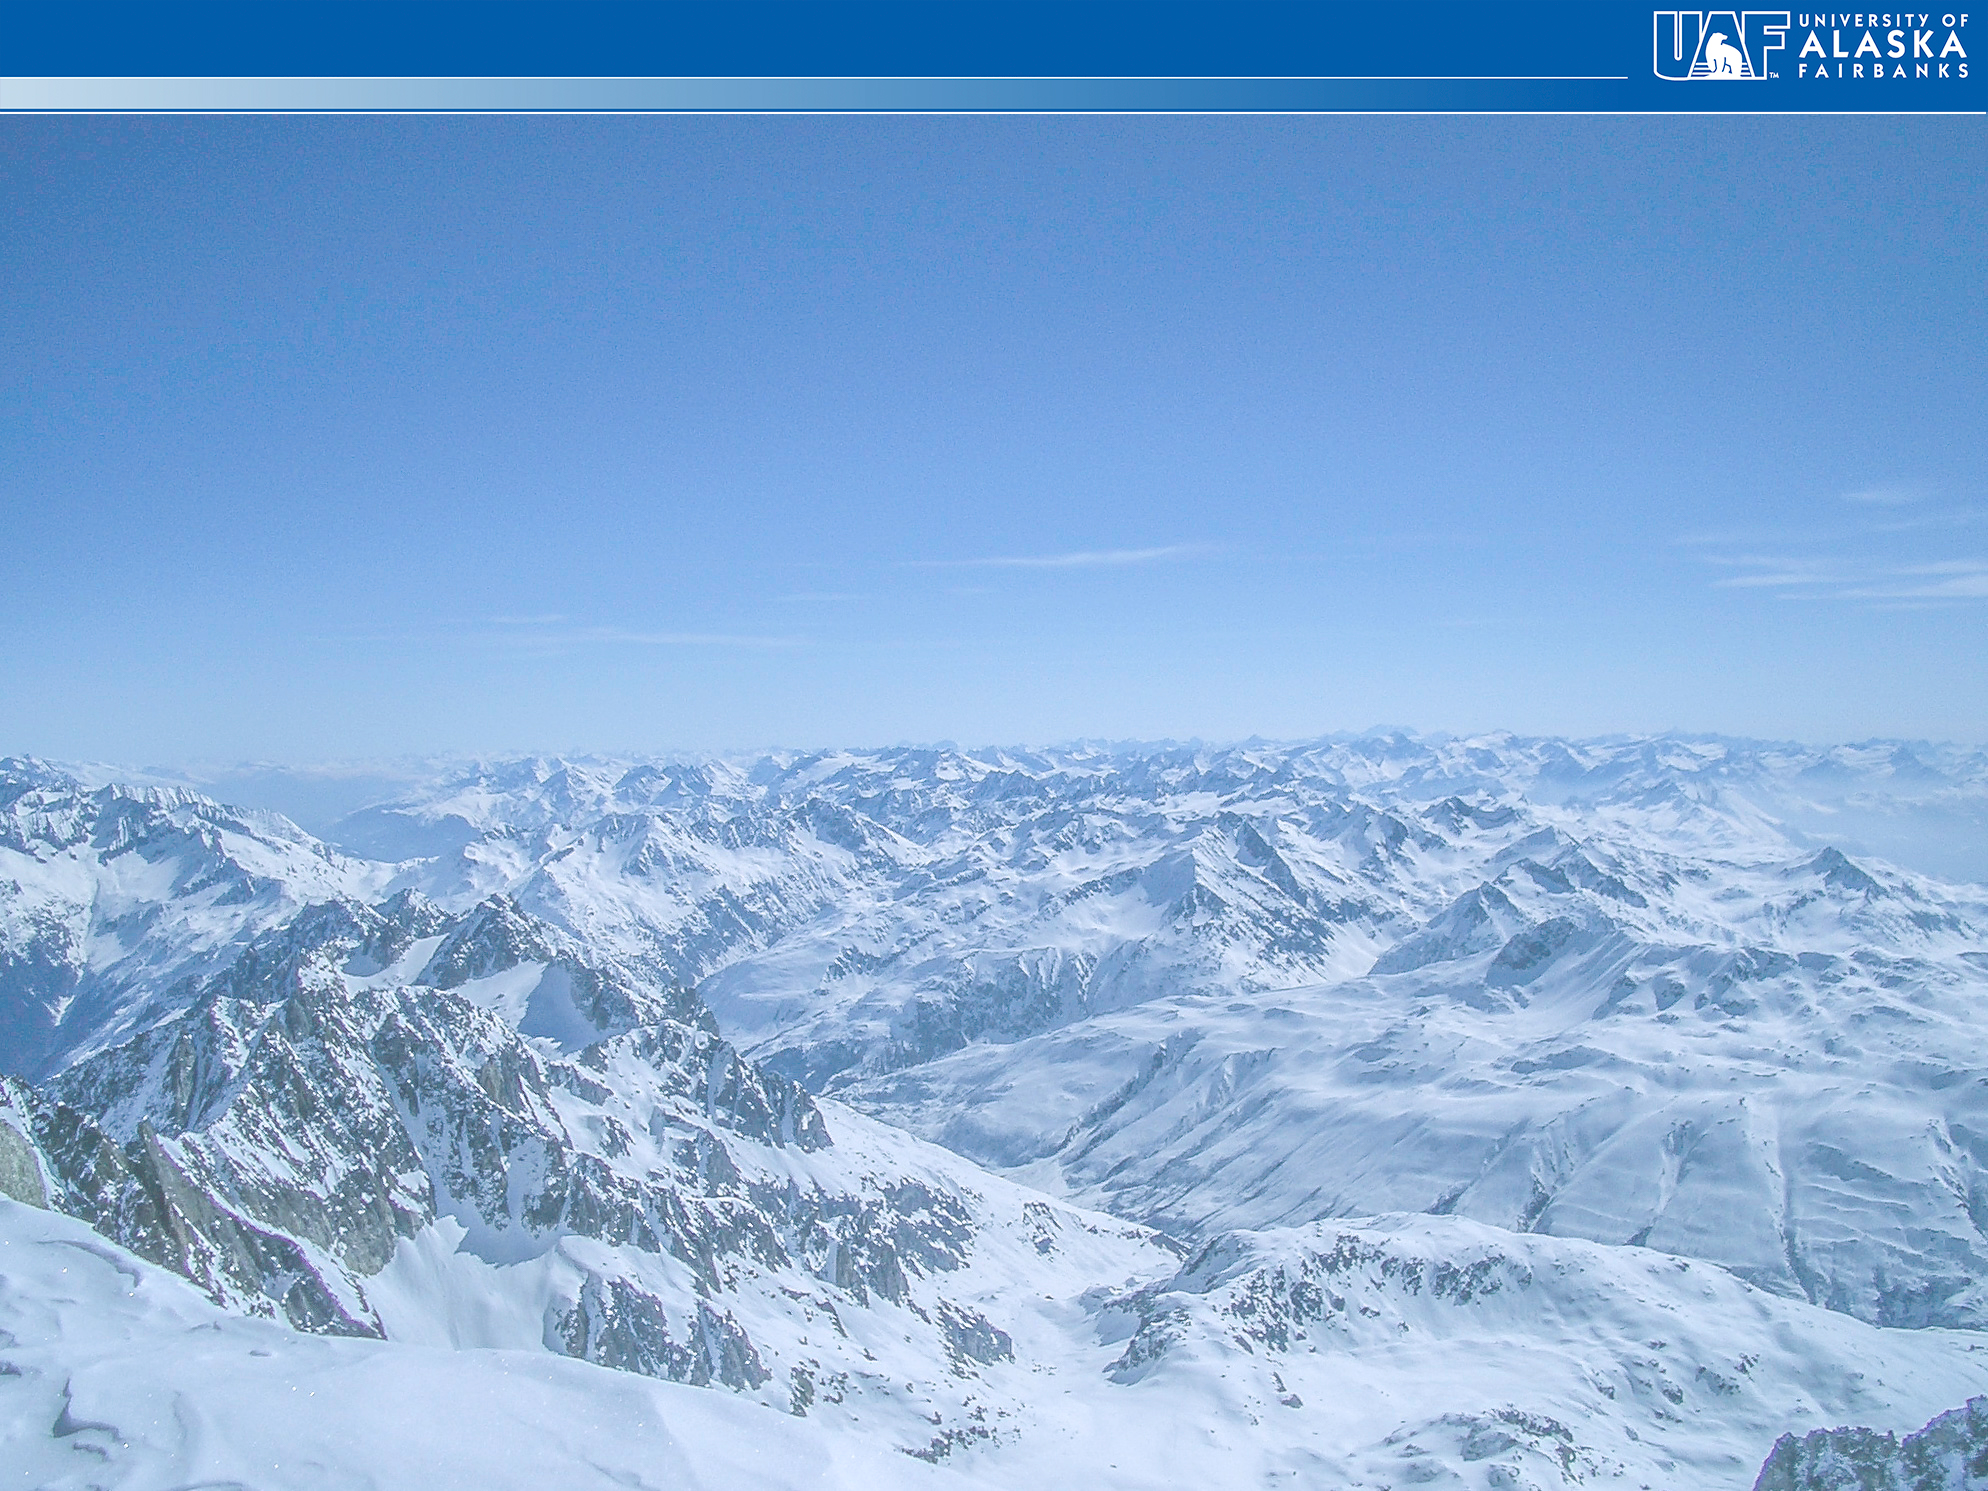
\includegraphics[width=\paperwidth]{galenstock_bg}};}
}

% insert titlepage
\begin{frame}
  \titlepage
  \note[item]{Who has ever seen a glacier?}
  \note[item]{Who has ever set foot on a glacier?}
  \note[item]{The picture here shows the view from on of my favorite places near}
  \note[item]{where I grew up}
\end{frame}

\setbeamertemplate{background canvas}
  {
} 


\setbeamertemplate{background canvas}
  {
     \tikz{\node[inner sep=0pt,opacity=1.] {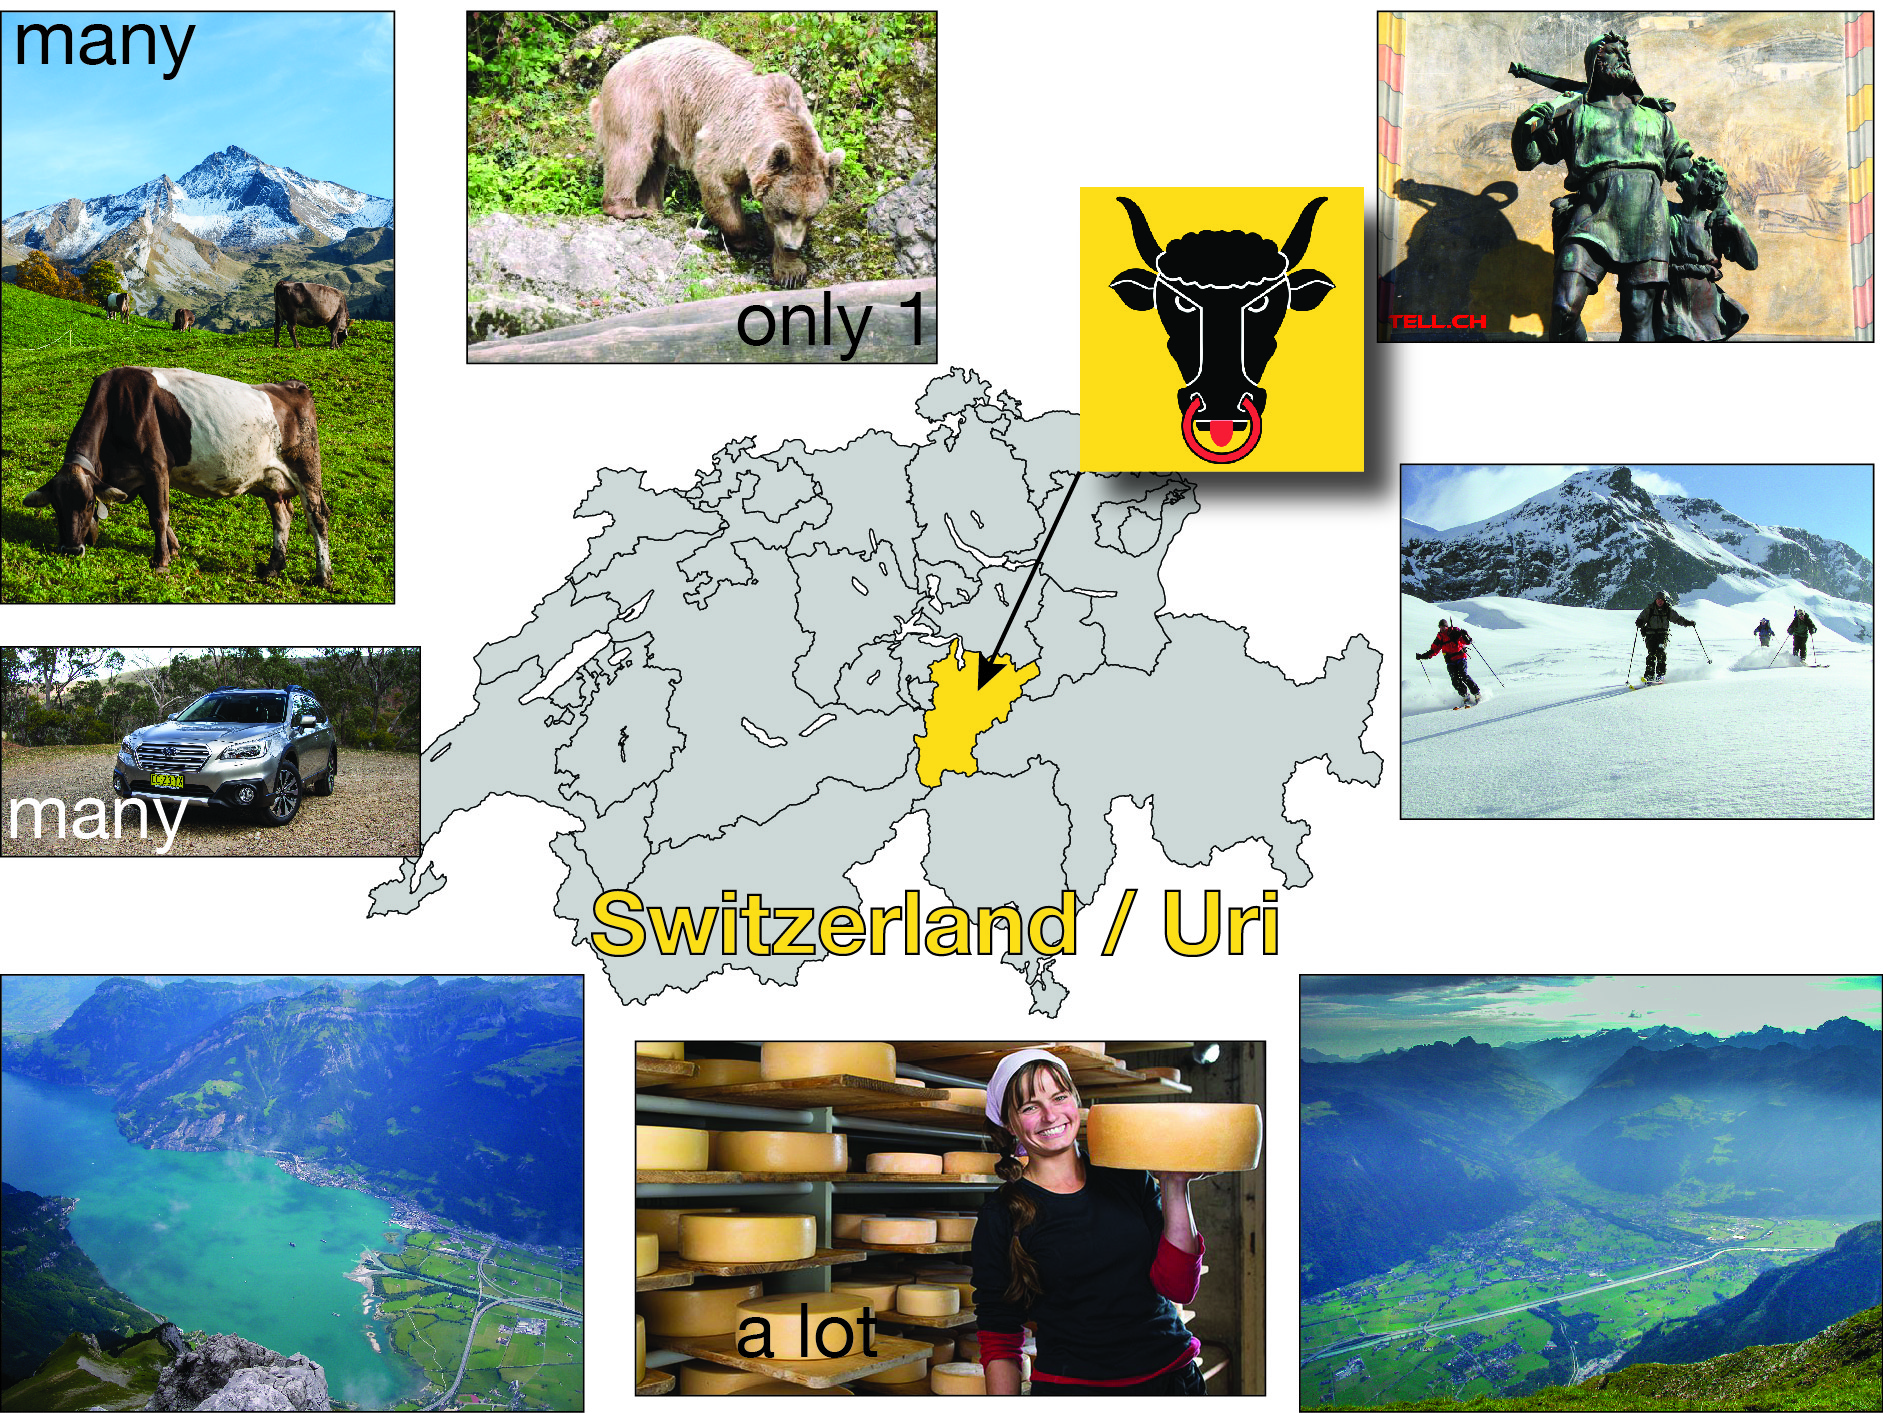
\includegraphics[width=\paperwidth]{uri-collage}};}
}

\begin{frame}[plain]
  \note[item]{I grew up in the heart of Switzerland, in the Kanton Uri---a Kanton is the equivalent to a State}
  \note[item]{Like Alaska, we have many Subarus}
  \note[item]{True to the stereotype, we have many cows in Uri and produce a lot of good cheese}
  \note[item]{Last year we had on bear roaming through Uri, which gave it some Alaska-feel}
  \note[item]{The last bear was shot in Uri in 1820 and you can still see the claws mounted to a house}
  \note[item]{According to legend, William Tell was born in Uri, who freed us from the Austrian oppression in 1291}
  \note[item]{But first and foremost have a lot of mountains to climb and to ski}
\end{frame}

\setbeamertemplate{background canvas}
{
  \tikz{\node[inner sep=0pt,opacity=1.] {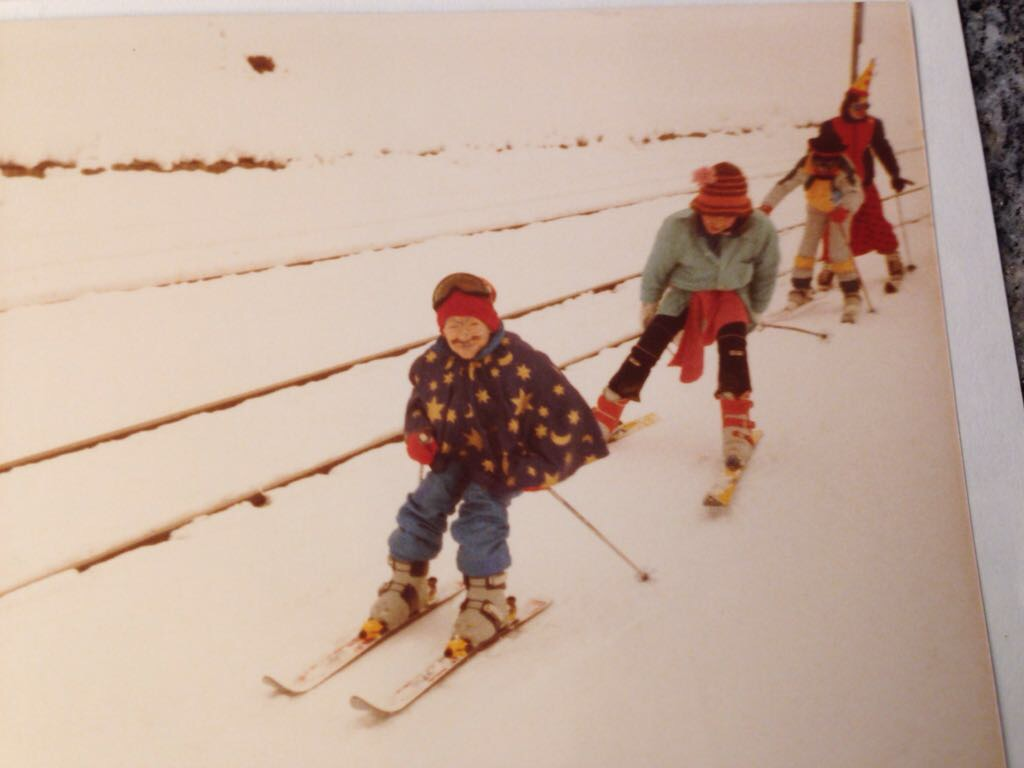
\includegraphics[width=\paperwidth]{andy-ski}};}
}

\begin{frame}[plain]
  \note[item]{So no surprise}
  \note[item]{I grew up on skis, I learned to downhill ski right after learning to walk}
  \note[item]{In Switzerland ``skiing'' always means downhill skiing, unlike here in Fairbanks where skiing usually means XC skiing}
\end{frame}



\setbeamertemplate{background canvas}
{
  \tikz{\node[inner sep=0pt,opacity=1.] {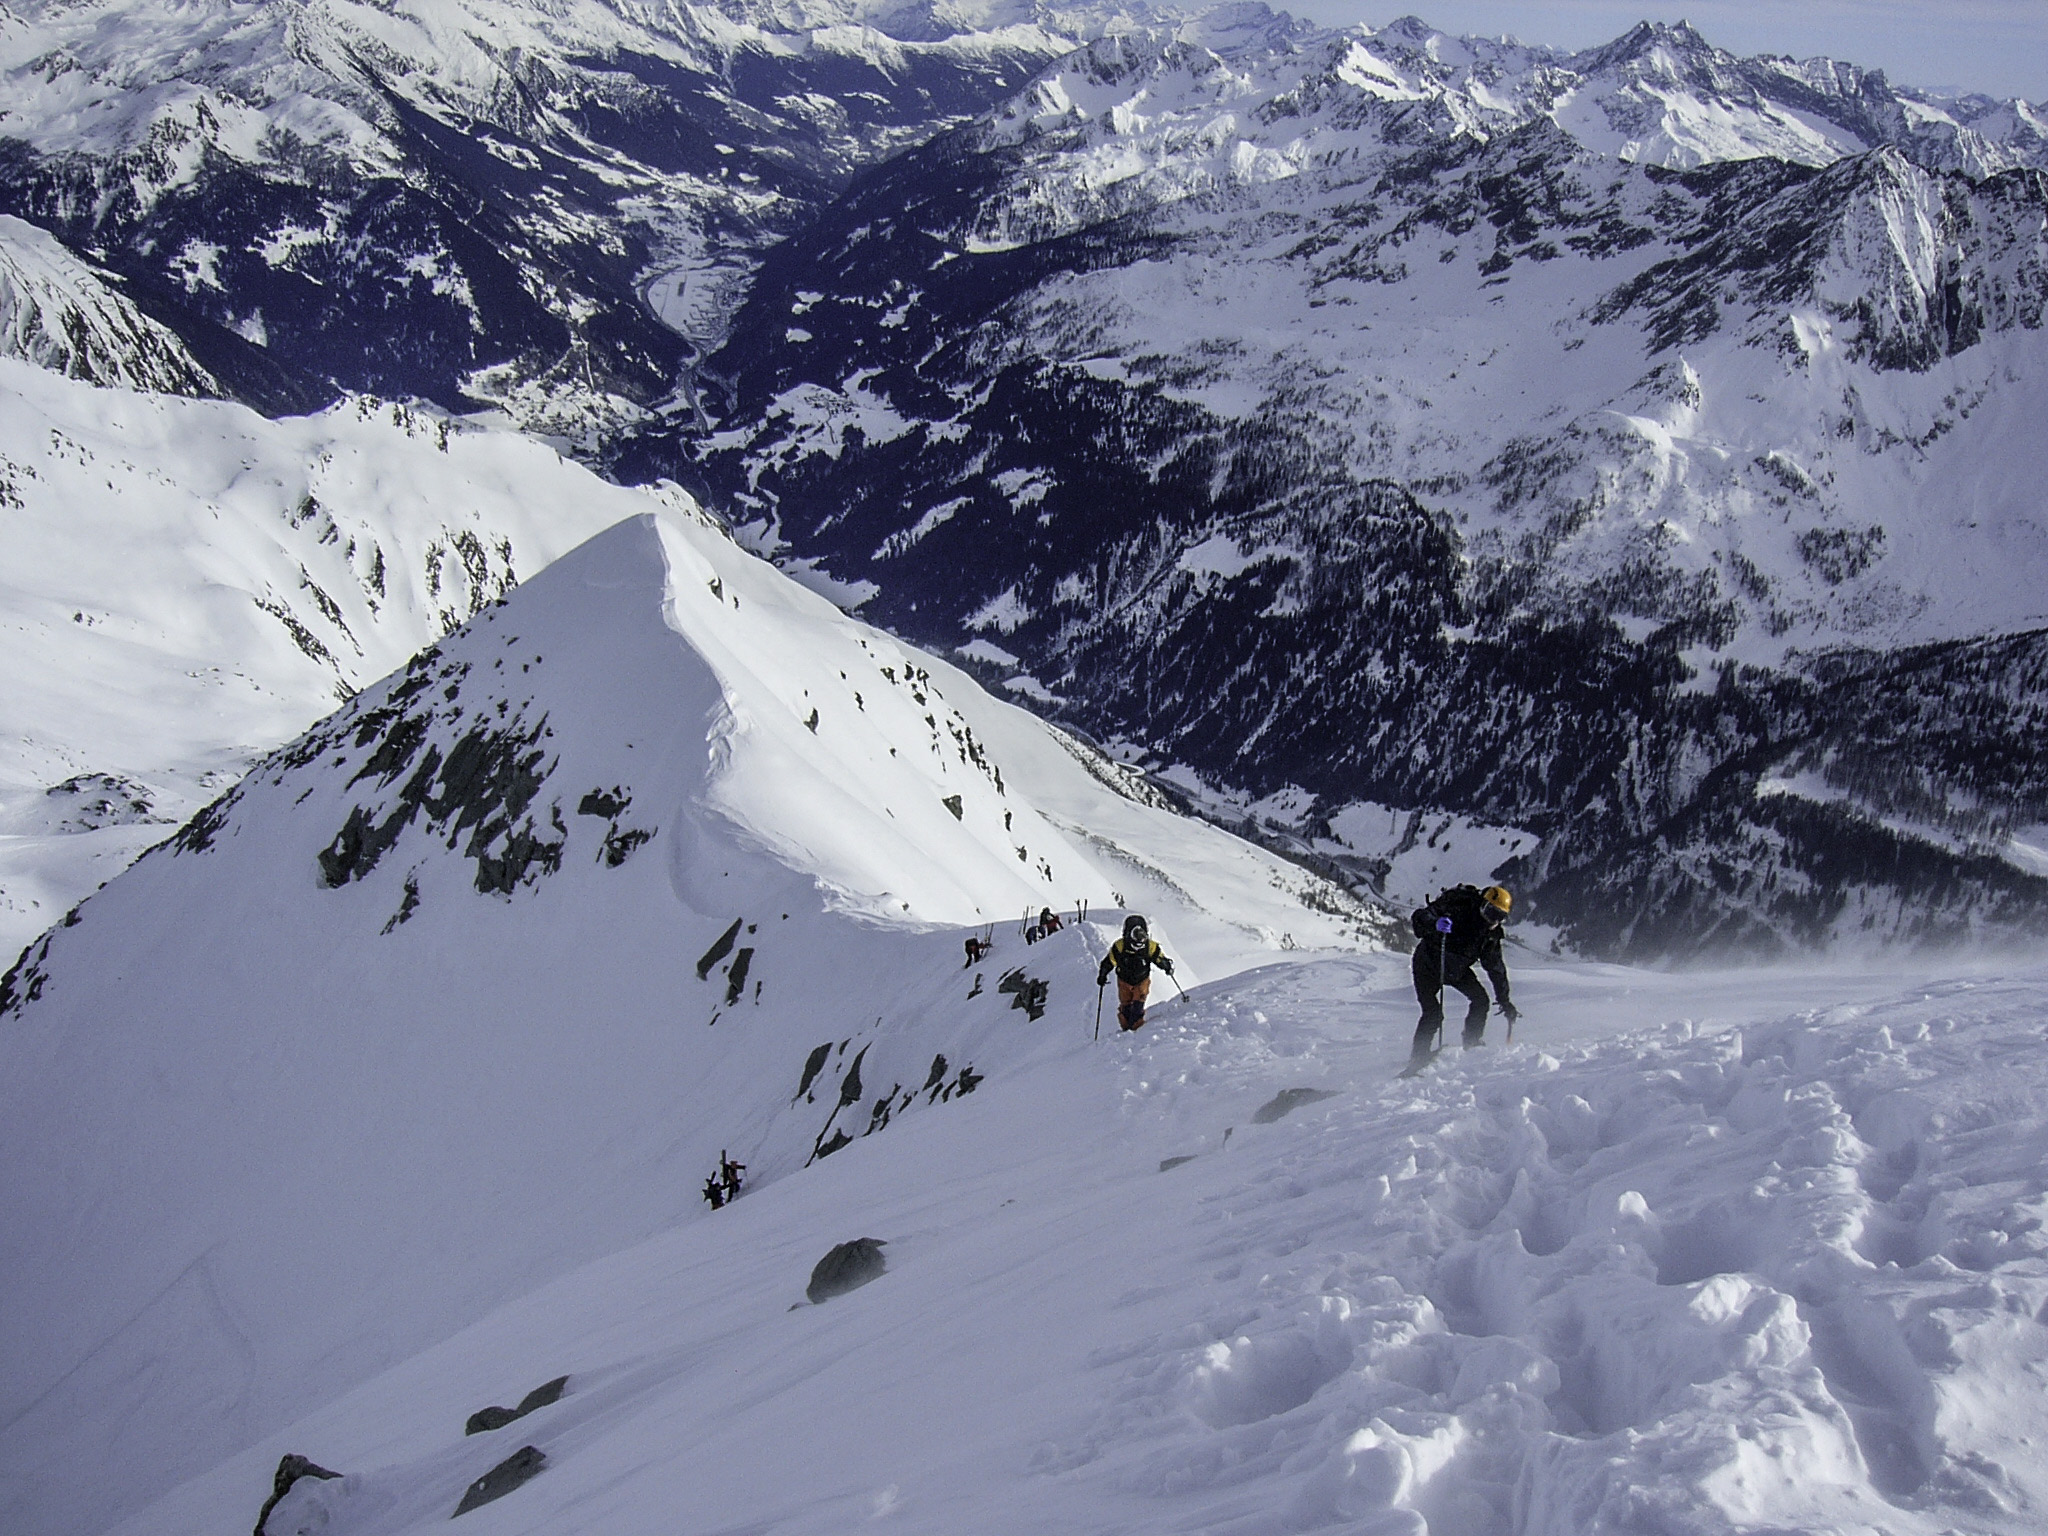
\includegraphics[width=\paperwidth]{ski-climb}};}
}

\begin{frame}[plain]
  \note[item]{When I was a bit older, I became tired of waiting for the next gondola}
  \note[item]{so started with ski mountaineering}
  \note[item]{and while spending my weekends in the mountains,}
  \note[item]{I started to notice change}
\end{frame}

\setbeamertemplate{background canvas}
{
  \tikz{\node[inner sep=0pt,opacity=1.] {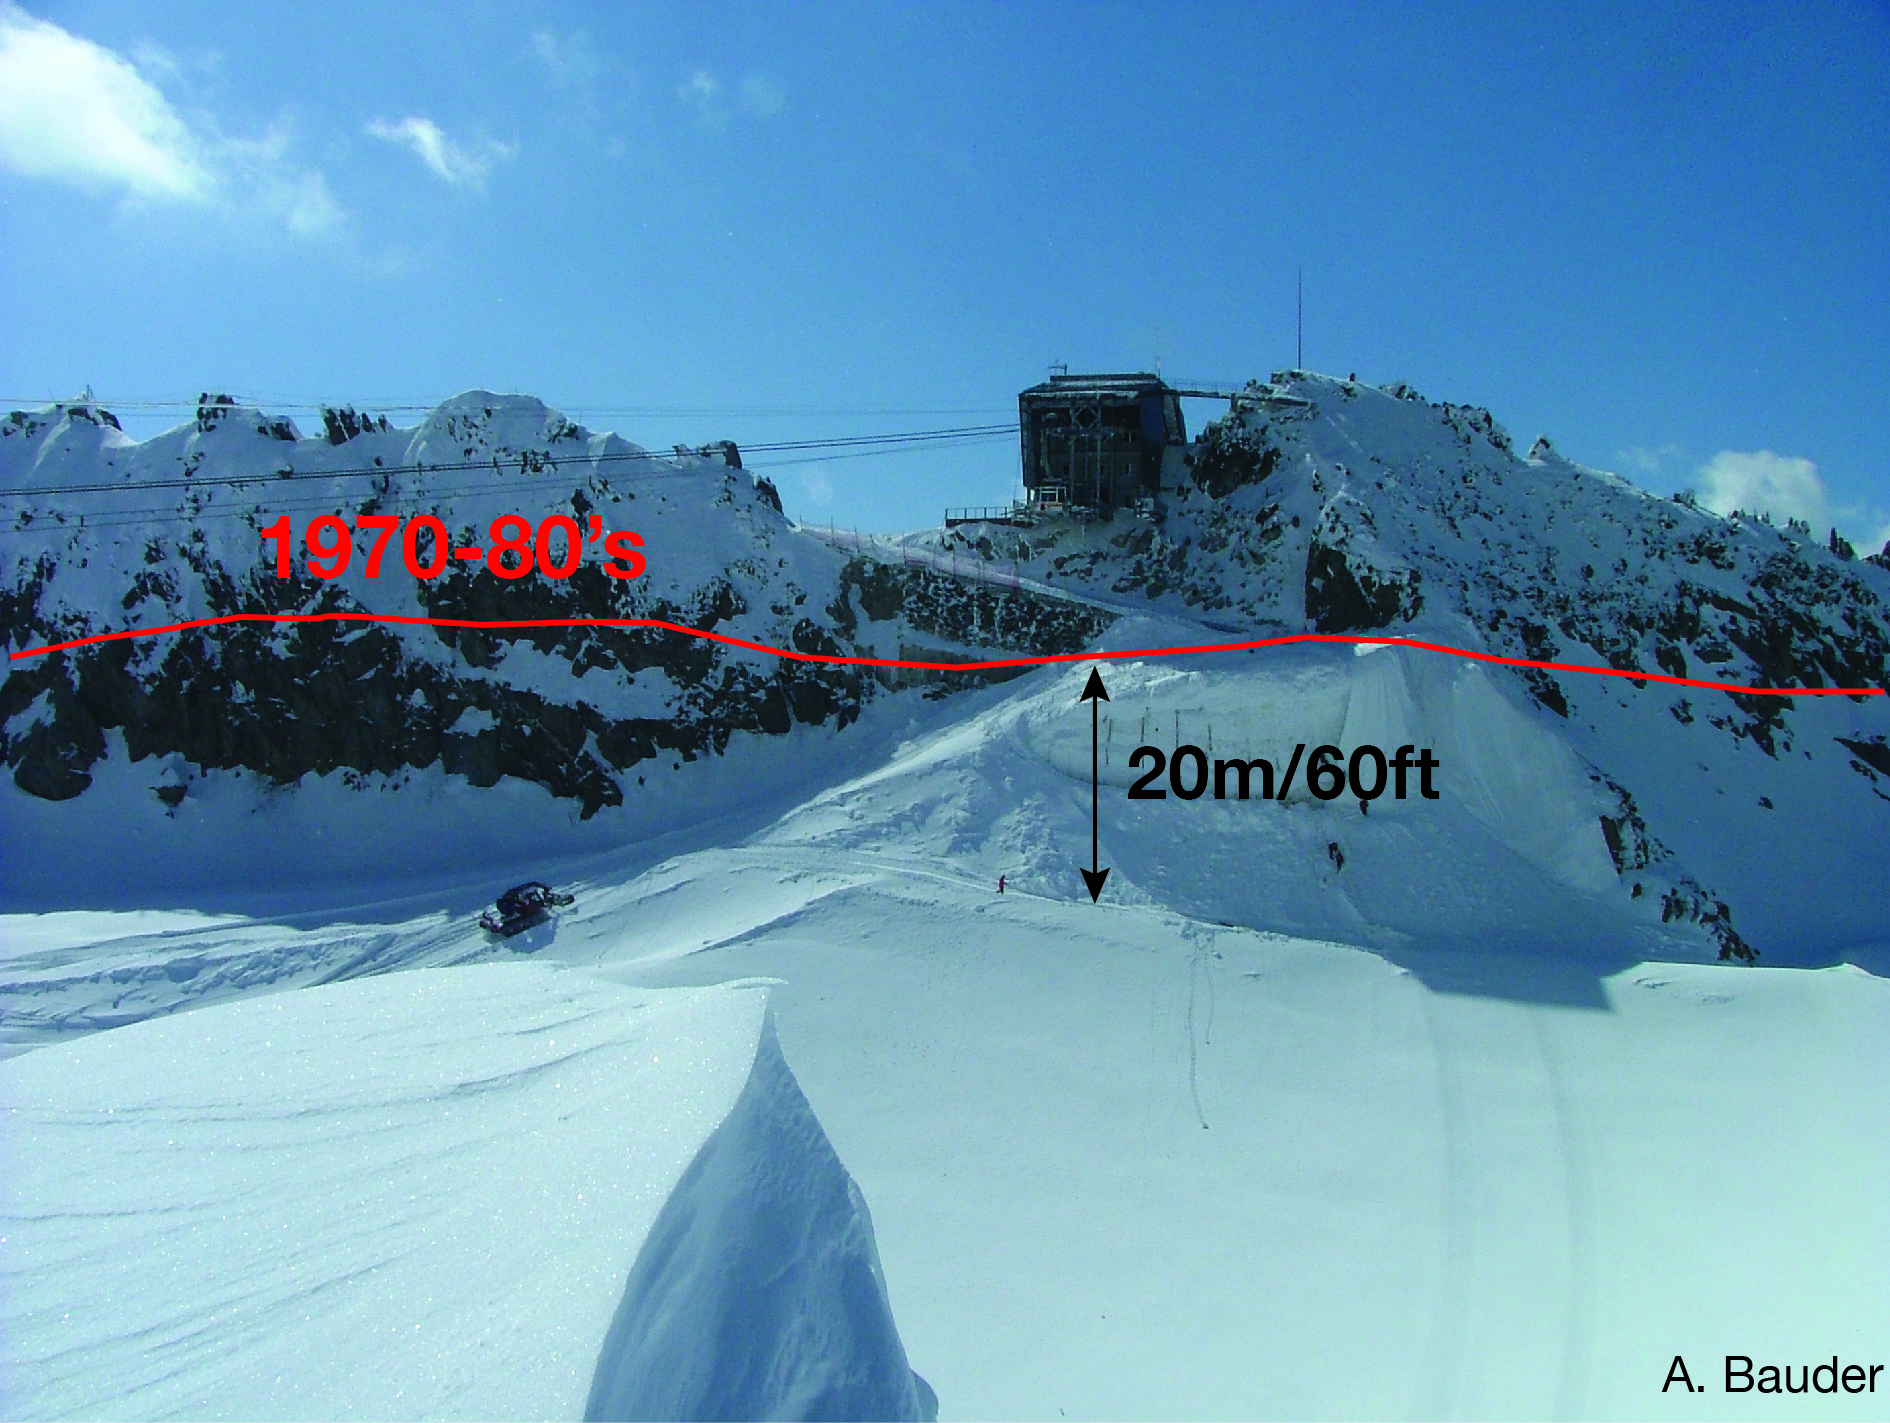
\includegraphics[width=\paperwidth]{gurschen-bauder}};}
}


\begin{frame}[plain]
  \note[item]{For example, when I was little we got out of the gondola}
  \note[item]{and we started to ski right on the glacier}
  \note[item]{However, in the past 2 or 3 decades, the glacier thinned by 20\,m or more}
  \note[item]{To get skiers on the glacier, they have to build a ramp out of snow every year}
  \note[item]{This is quite labor intensive and requires a lot of gas}
  \note[item]{Now, every spring ski patrol covers the ramp with a white tarp to preserve as much as possible}
  \note[item]{for the next winter}
  \note[item]{I asked myself: Are glaciers melting only where I grew up or is there more to it?}
  \note[item]{Is this happens somewhere else?}
  \note[item]{so, to answer this, I decided to study glaciers and climate}
  \note[item]{but also it sounded like fun to study something that I can ski on\ldots}
  \note[item]{So during the rest of talk, I would like to give you my perspective of glaciers and glacier change}
  \note[item]{I will tell you about the health of Alaska's glaciers}
  \note[item]{and why we glaciologists are so concerned about WAIS}
\end{frame}
  

\setbeamertemplate{background canvas}
{
} 


\begin{frame}{Glaciers in Alaska}
  \begin{figure}
    \includegraphics<1>[width=1\textwidth]{gulkana1967}
    \includegraphics<2>[width=1\textwidth]{gulkana2016}
    \includegraphics<3>[width=1\textwidth]{gulkana2016-line}
    {\\ Fifty Years of Glacier Change in Alaska; USGS}
  \end{figure}
  \note[item]{Gulkana thinned and retreated}
\end{frame}


\begin{frame}{Glaciers in Alaska}
  \flashmovie[width=15cm]{documenting_glacial_change.swf}
  \url{http://serc.carleton.edu/eslabs/cryosphere/5a.html}
  \note[item]{I found a great website illustrating glacier change}
  \note[item]{where you can go and see for yourself}
  \note[item]{Couldn't make it bigger.}
\end{frame}


\setbeamertemplate{background canvas}
{
  \tikz{\node[inner sep=0pt,opacity=1]{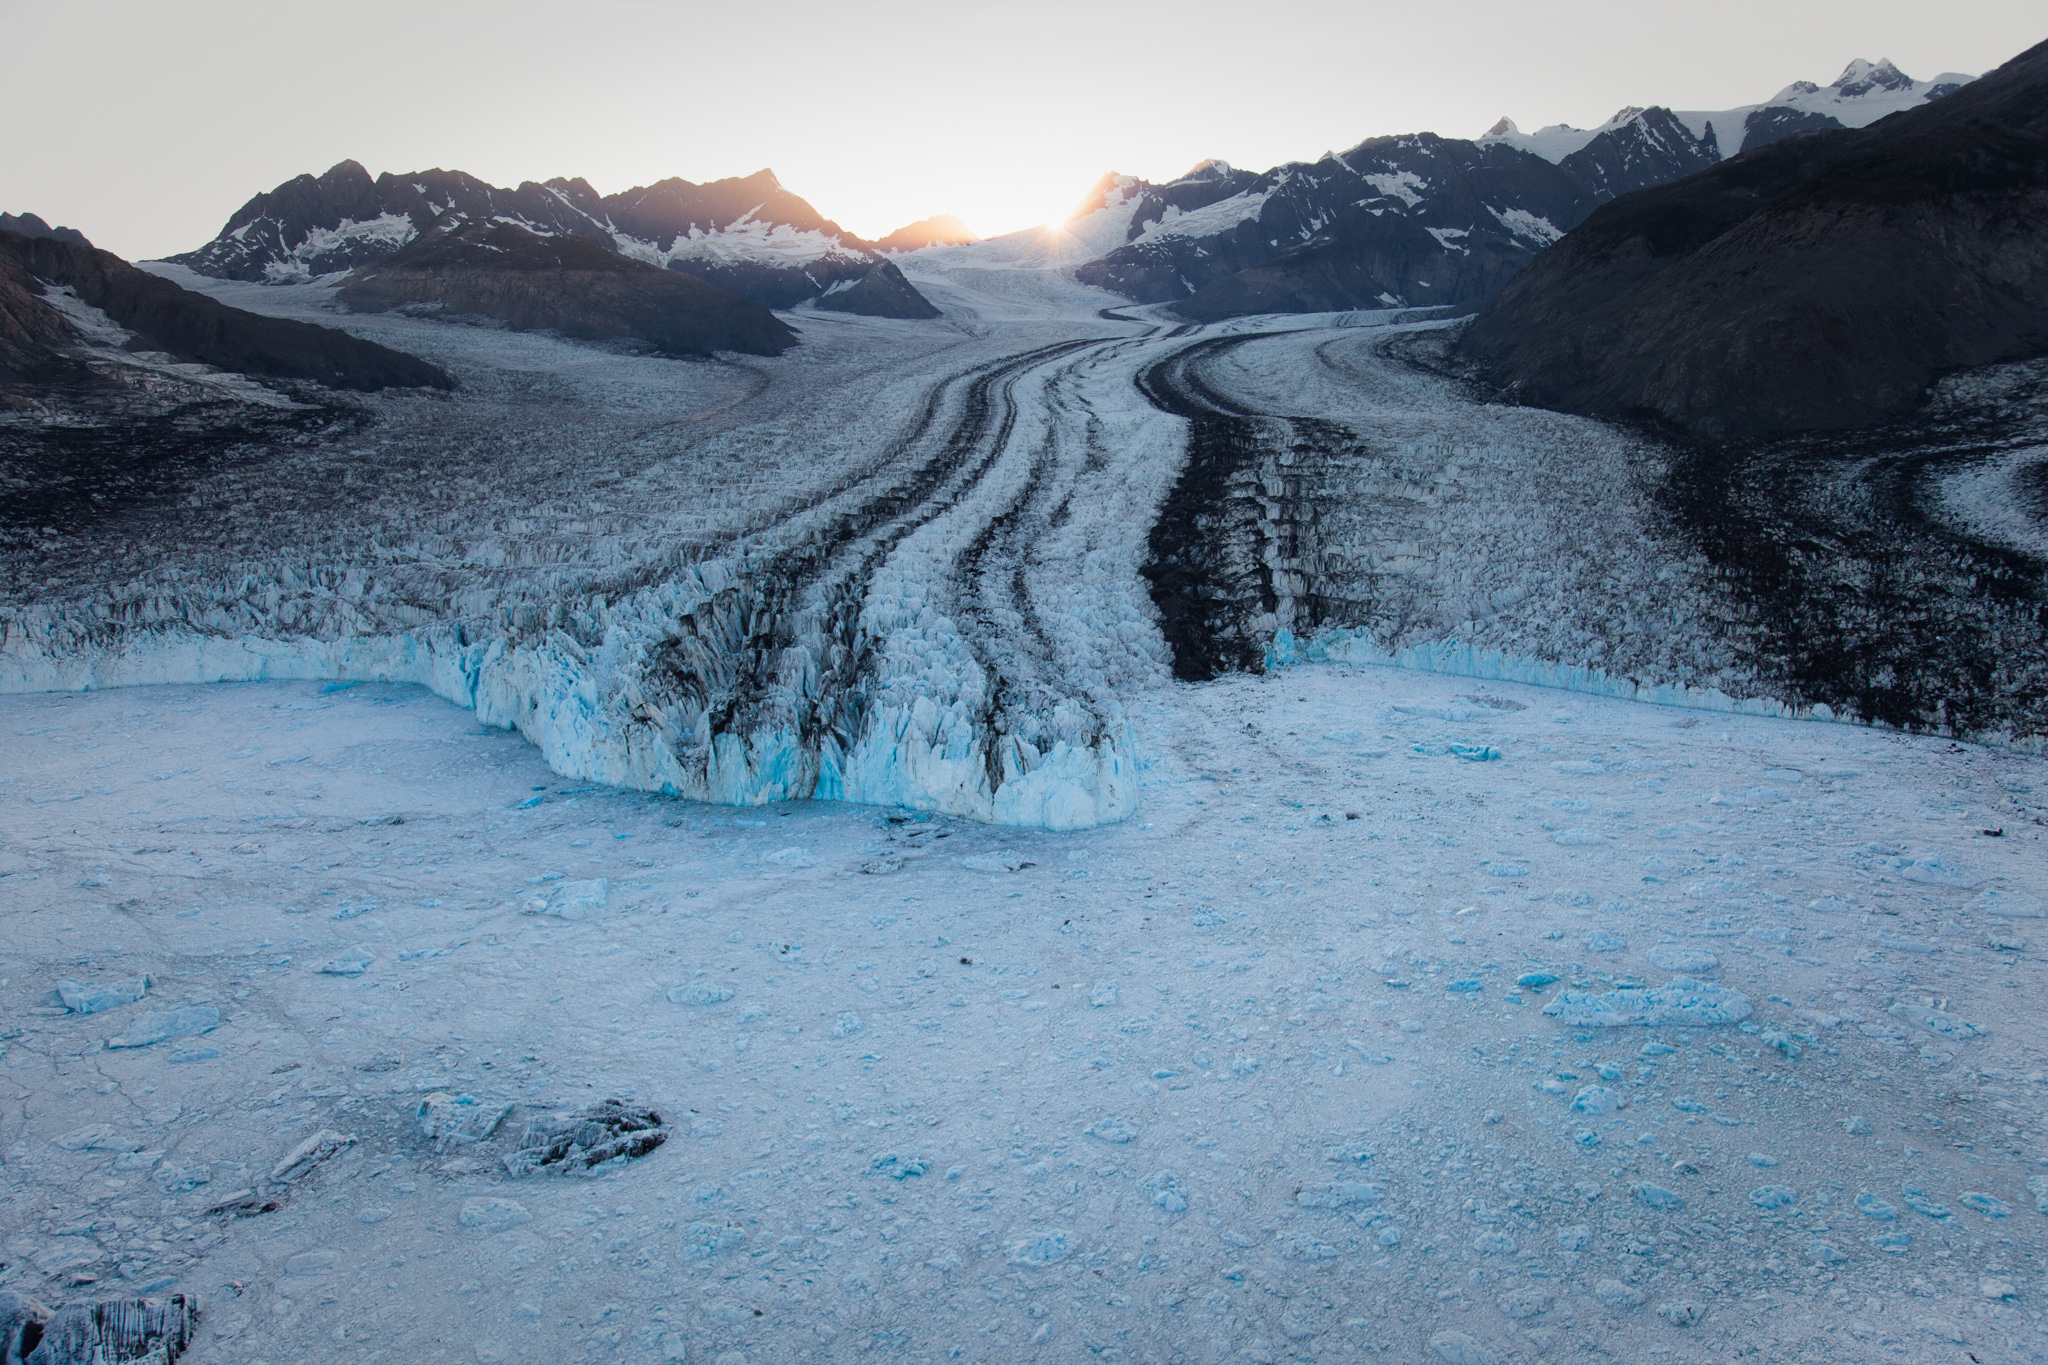
\includegraphics[width=\paperwidth,height=\paperheight]{columbia-glacier-2010}};}
}

\begin{frame}{Columbia Glacier}
  \note[item]{Who has been to Columbia Glacier near Valdez?}
  \note[item]{The photo here it took from an Alaska Tourism website and it dates to 2010.}
  \note[item]{You can see Columbia Glacier flowing into the ocean}
  \note[item]{The vertical cliff here is called the glacier terminus or the calving front}
\end{frame}

\setbeamertemplate{background canvas}
{
}



\begin{frame}{Melting Glaciers in Alaska: Columbia Glacier}
  \begin{figure}
   \movie[showcontrols=true,autostart,loop,width=12cm]{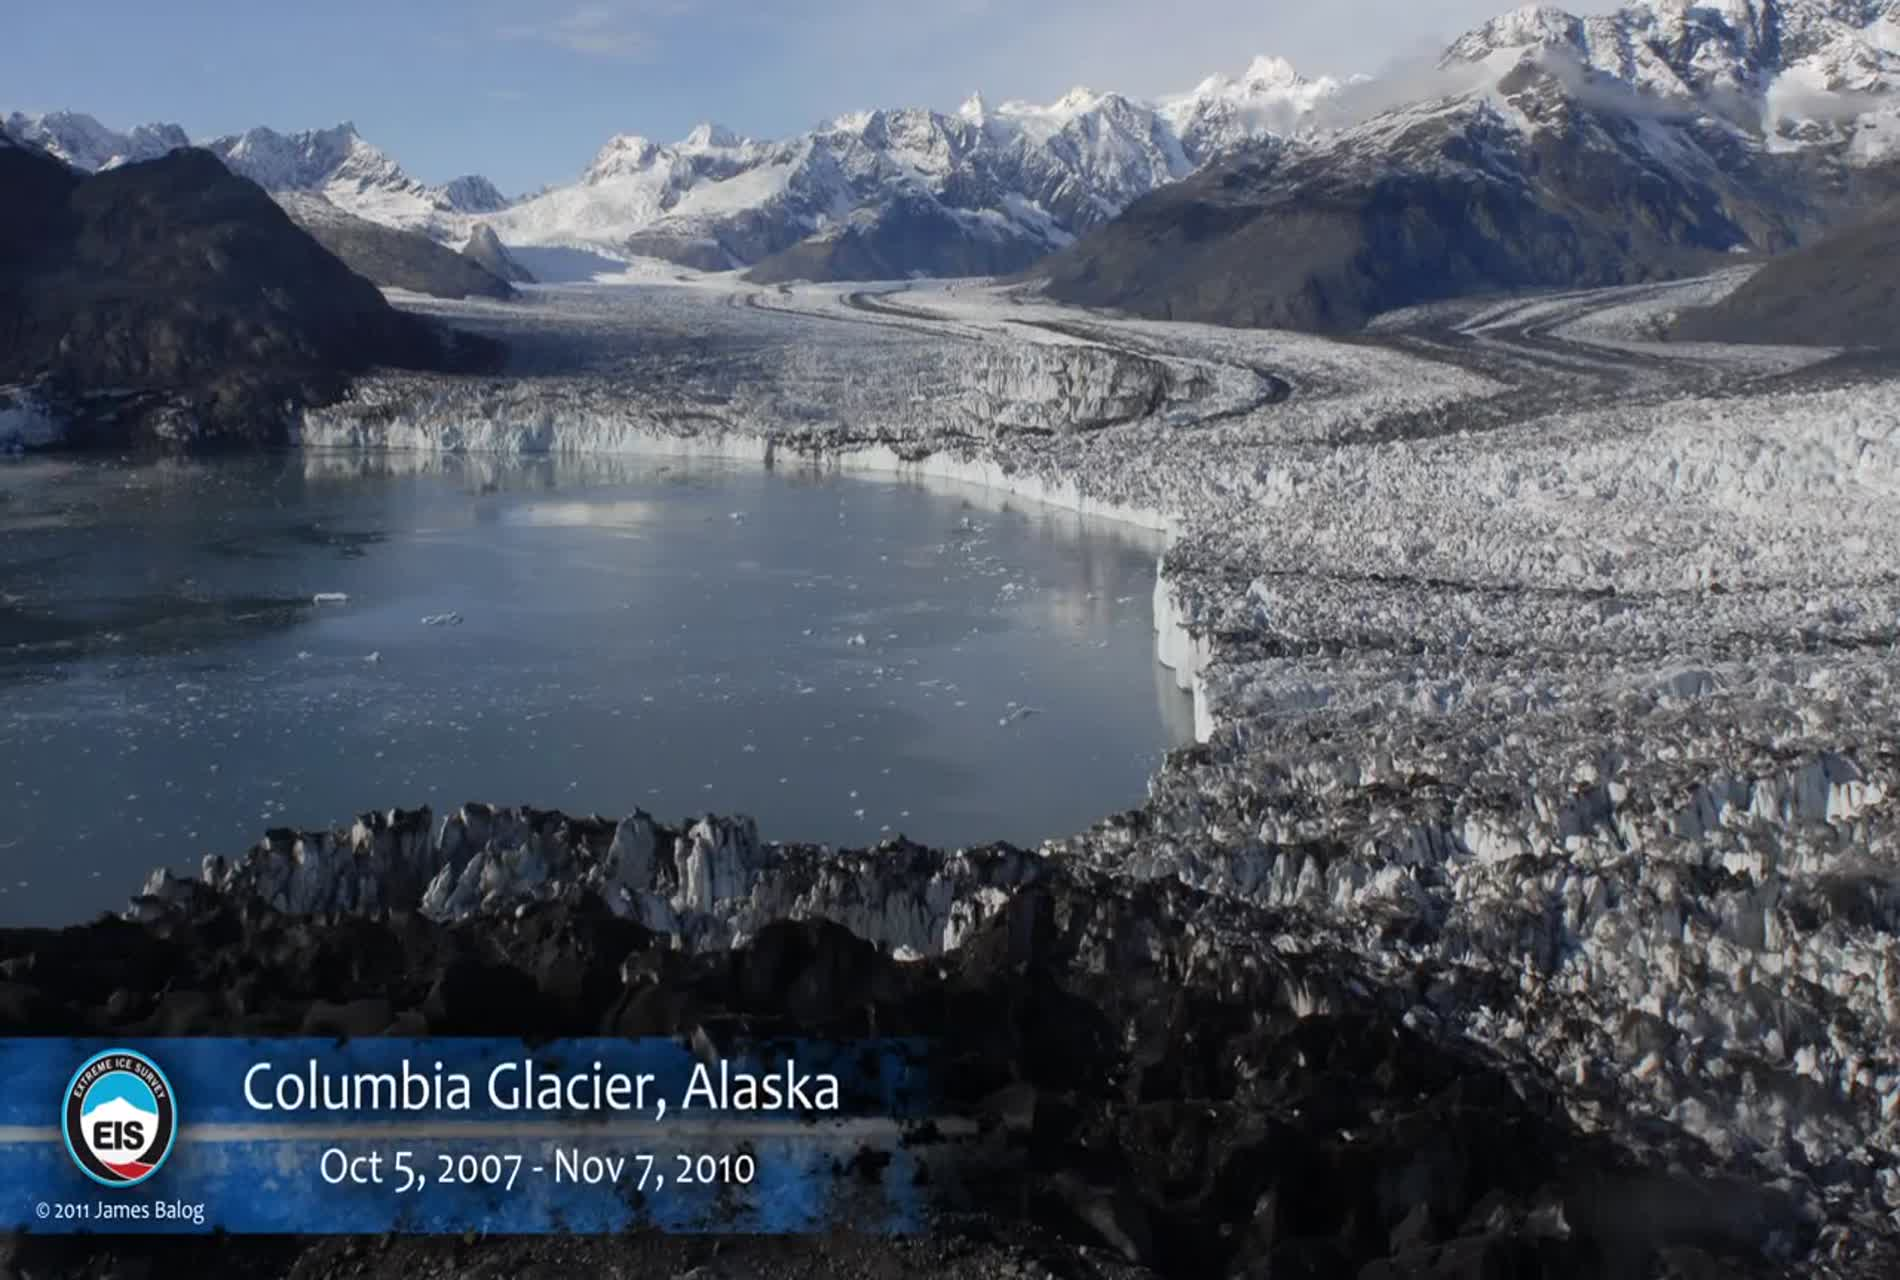
\includegraphics[width=12cm]{columbia-eis}}{columbia-eis.mov}
  \end{figure}
  \note[item]{Here is a video put together from time lapse photography by James Balog from EIS.}
  \note[item]{Columbia Glacier looks like a river of frozen ice, all cracked up, flowing into the ocean}
  \note[item]{When Columbia Glacier was first surveyed by British explorers in 1794}m
  \note[item]{it extented to Heather Bay and held that position until 1980.}
  \note[item]{In 1980s, Columbia Glacier started a rapid that continues today.}
  \note[item]{Since 1986, Colmbia Glacier retreated by more than 20 kilometers.}
  \note[item]{It shows how fast the glacier retreated between 2007 and 2010.}
  \note[item]{In fact, Columbia Glacier retreated so fast}
  \note[item]{that they had to reposition the camera three times}
\end{frame}


\setbeamertemplate{background canvas}
{
  \tikz{\node[inner sep=0pt,opacity=0.75] {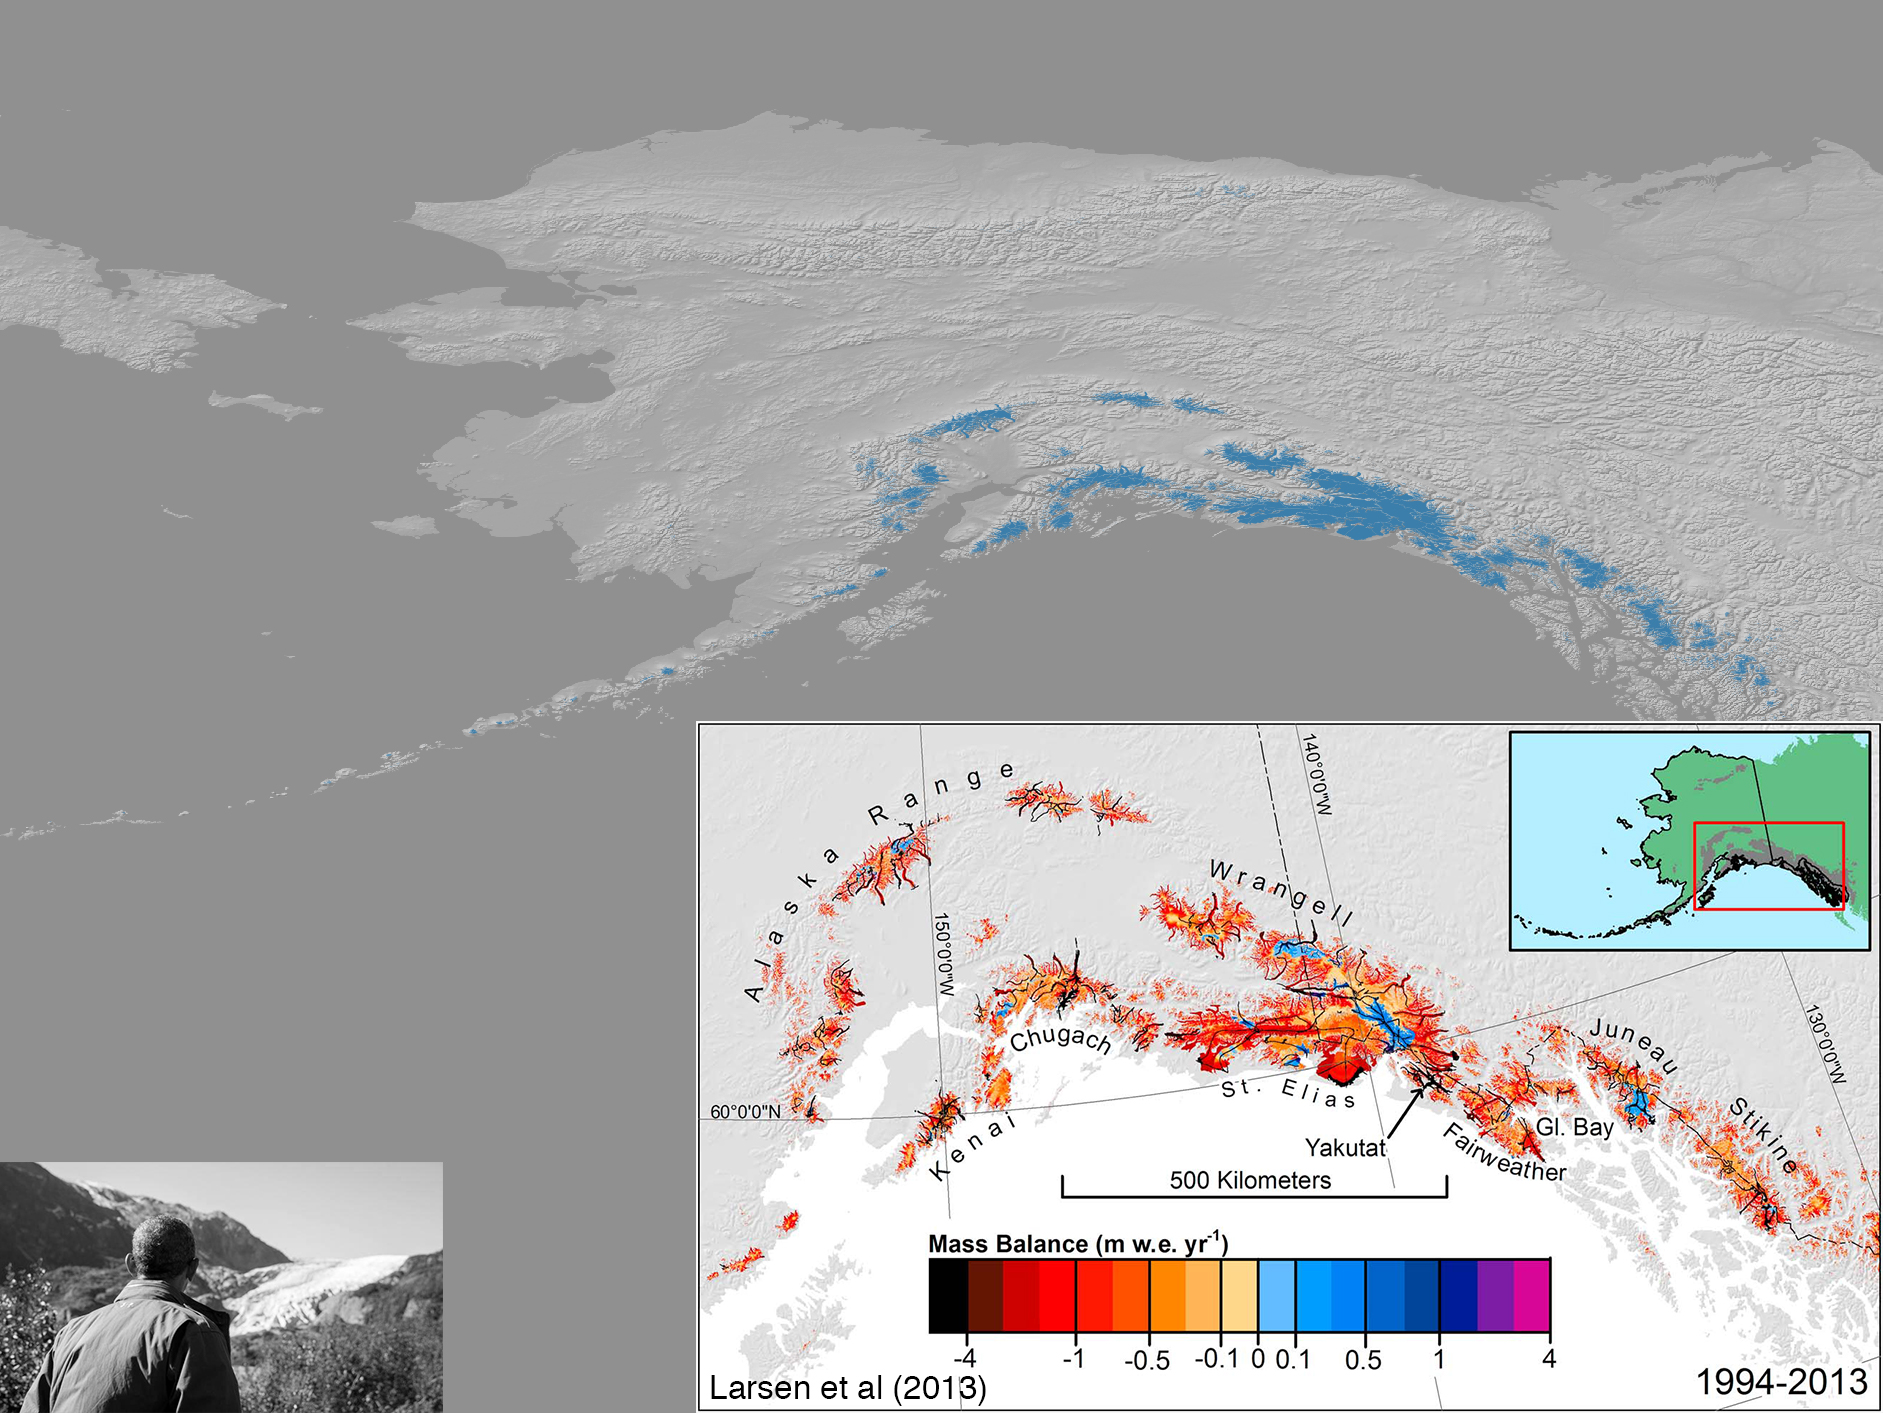
\includegraphics[width=\paperwidth]{ak_glacierized_area_melt_16x12}};}
}

\begin{frame}{Melting Glaciers in Alaska}
  \begin{itemize}
  \item total mass loss 1994--2013 from AK glaciers: 75$\pm$11 Gt/yr loss $\Rightarrow$ 5\,cm (2\,in) layer of water covering Alaska
  \end{itemize}
  \note[item]{Explain thinning and mass loss}
  \note[item]{Columbia Glacier is not alone}
  \note[item]{As recent study by UAF's Chris Larsen and others shows that many glaciers are melting}
  \note[item]{The red colors indicate glaciers that have lost mass between 1994 and 2013}
  \note[item]{while blue color indicate mass gain}
  \note[item]{there are many more glaciers losing mass than gaining mass}
  \note[item]{Between 94 and 2013, Alaskan glaciers lost a combined 75 Gt per year}
  \note[item]{How much are 75 giga ton?}
  \note[item]{If you spread 75 Gt of water evenly over Alaska}
  \note[item]{and here we assume Alaska is flat}
  \note[item]{we would stand in 5cm deep water}
  \note[item]{or, if we combine all 20 years, would be standing in about a meter of water}

\end{frame}

\setbeamertemplate{background canvas}
{
}



\begin{frame}{Melting Glaciers Everywhere: The Biggest Losers}
  \begin{figure}
    {Alaska \qquad---\qquad West Greenland \qquad---\qquad West Antartica}
    \\[1em]
    \includegraphics<1>[width=1\textwidth]{world-grace-2002-2016}
  \end{figure}
  \note[item]{But maybe Switzerland and Alaska are the exception?}
  \note[item]{Glaciers are melting worldwide}
  \note[item]{This figure shows glacier mass loss world wide}
  \note[item]{Again, red colors indicate mass loss}
  \note[item]{The biggest red areas are Alaska, Greenland, and West Antartica}
  \note[item]{These are the biggest losers right now}
\end{frame}

\setbeamertemplate{background canvas}
{
  \tikz{\node[inner sep=0pt,opacity=.6] {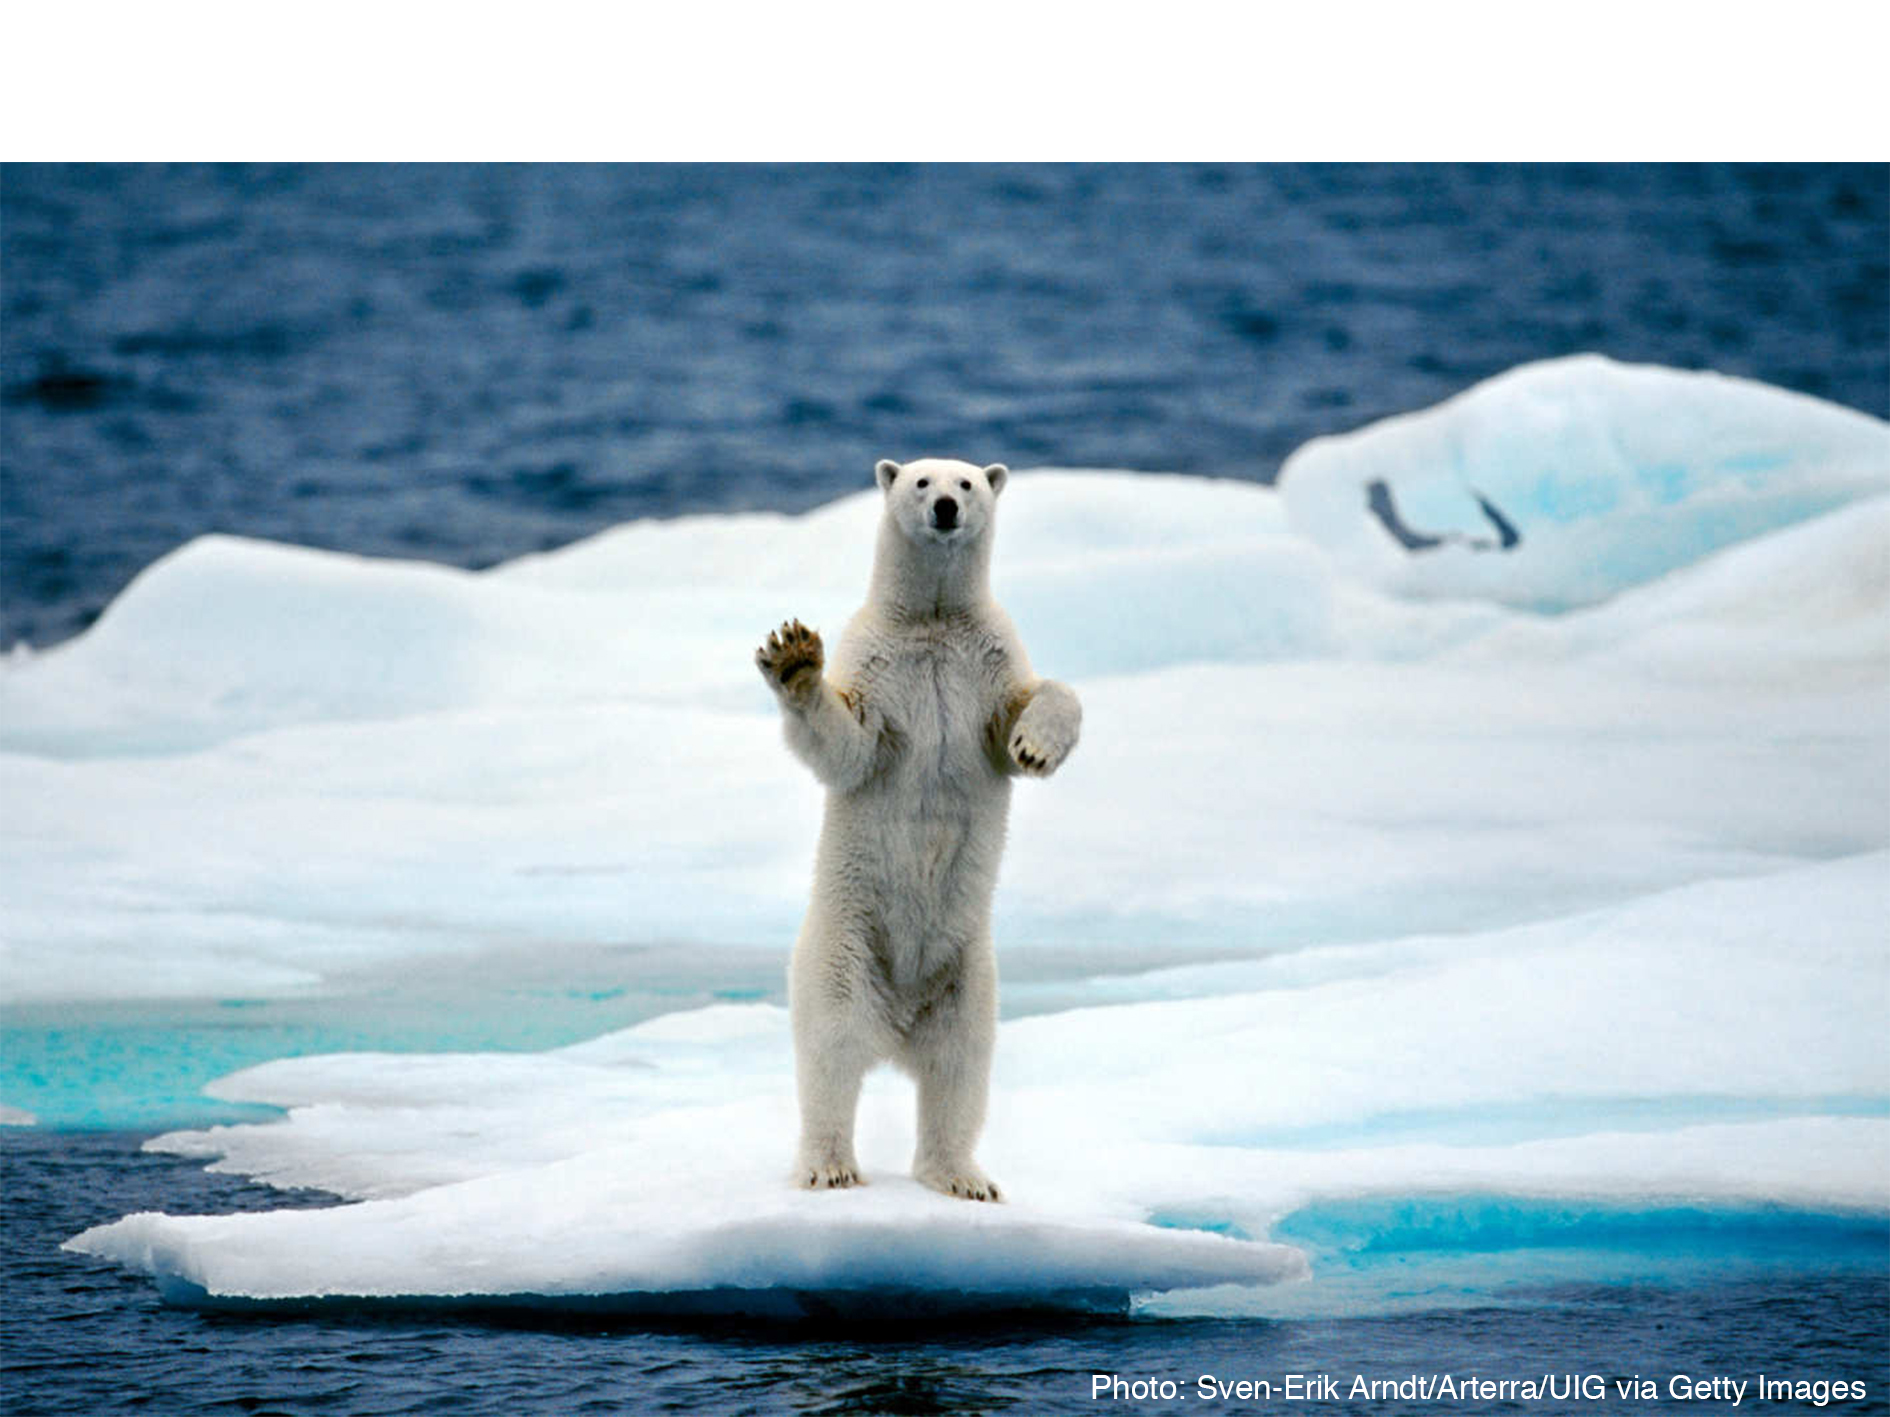
\includegraphics[height=\paperheight,width=\paperwidth]{polar-bear-wcredit}};}
}


\begin{frame}{}
  \centering{``Hasn't the Climate Changed Before?''}
  \note[item]{But wait}
  \note[item]{aren't glaciers and the climate constantly changing}
  \note[item]{What's so special about today?}
  \note[item]{That's probably the number one question}
  \note[item]{I get from a seat neighbor in airplane}
  \note[item]{So let me try to walk you through the climate of the past}
  \note[item]{and how the climate influences glaciers}
\end{frame}

\setbeamertemplate{background canvas}
{
}


\begin{frame}{Glacials and Interglacials}
      \begin{figure}
        \includegraphics<1>[height=8.2cm]{ice-age-movies}
      \end{figure}
  \note[item]{As we learned from Hollywood}
  \note[item]{there have been Ice Ages and Meltdowns}
  \note[item]{or as we call it: glacials and interglacials}
\end{frame}

\setbeamertemplate{background canvas}
{
  \tikz{\node[inner sep=0pt,opacity=1] {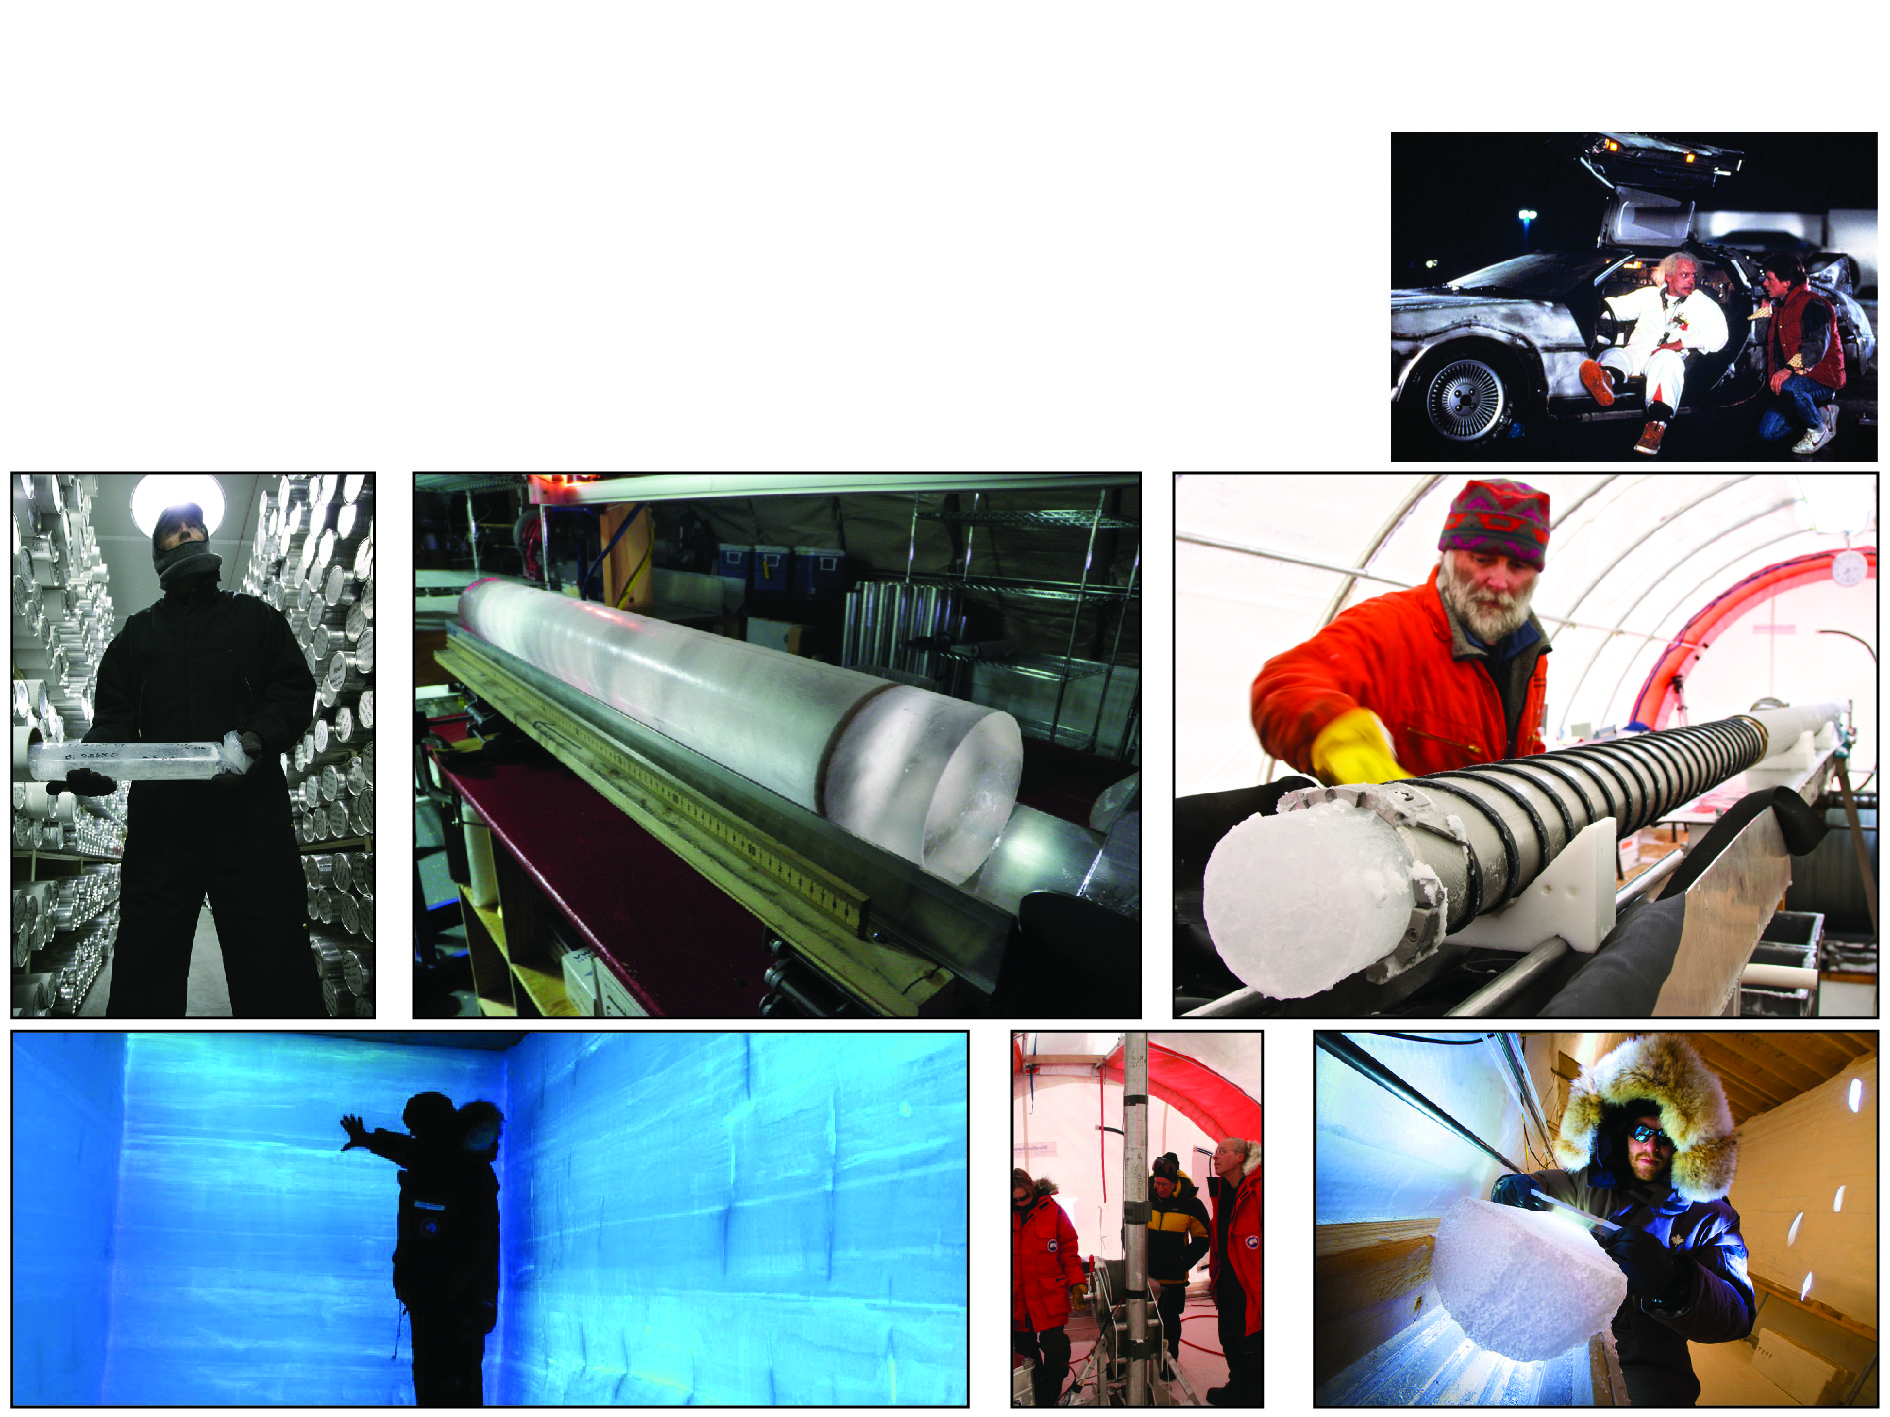
\includegraphics[height=\paperheight,width=\paperwidth]{ice-core-collage}};}
}

\begin{frame}{Ice Cores: The 2-mile Time Machine}
  \note[item]{We know about glacials and interglacials from}
  \note[item]{geologic evidence and from ice cores}
  \note[item]{What is an ice core and what can it do for you?}
  \note[item]{In cold areas such as Greenland and Antarctica}
  \note[item]{snow falls every year on top of the snow from the previous year}
  \note[item]{building layer after layer, as you can see in the photo here}
  \note[item]{when the weight of the overlying snow is heavy enough, the snow turns into ice}
  \note[item]{during the process, tiny bubbles of air are being trapped within the ice}
  \note[item]{the air in those bubbles contains a lot of information}
  \note[item]{about the climate of the year when the snow fell}
  \note[item]{An ice cores are like a big archive that}
  \note[item]{stores information about past climate}
  \note[item]{each bubble is a time capsule}
  \note[item]{Ice cores from Greenland and Antartica are up to 2 mile deep}
  \note[item]{the deeper you go, the older the ice gets}
  \note[item]{climate scientists have analyzed ice that is up to 800,000 years old}
  \note[item]{This gives us a pretty good picture about climate varibility over almost a million years}
\end{frame}

\setbeamertemplate{background canvas}
{
  \tikz{\node[inner sep=0pt,opacity=0.4] {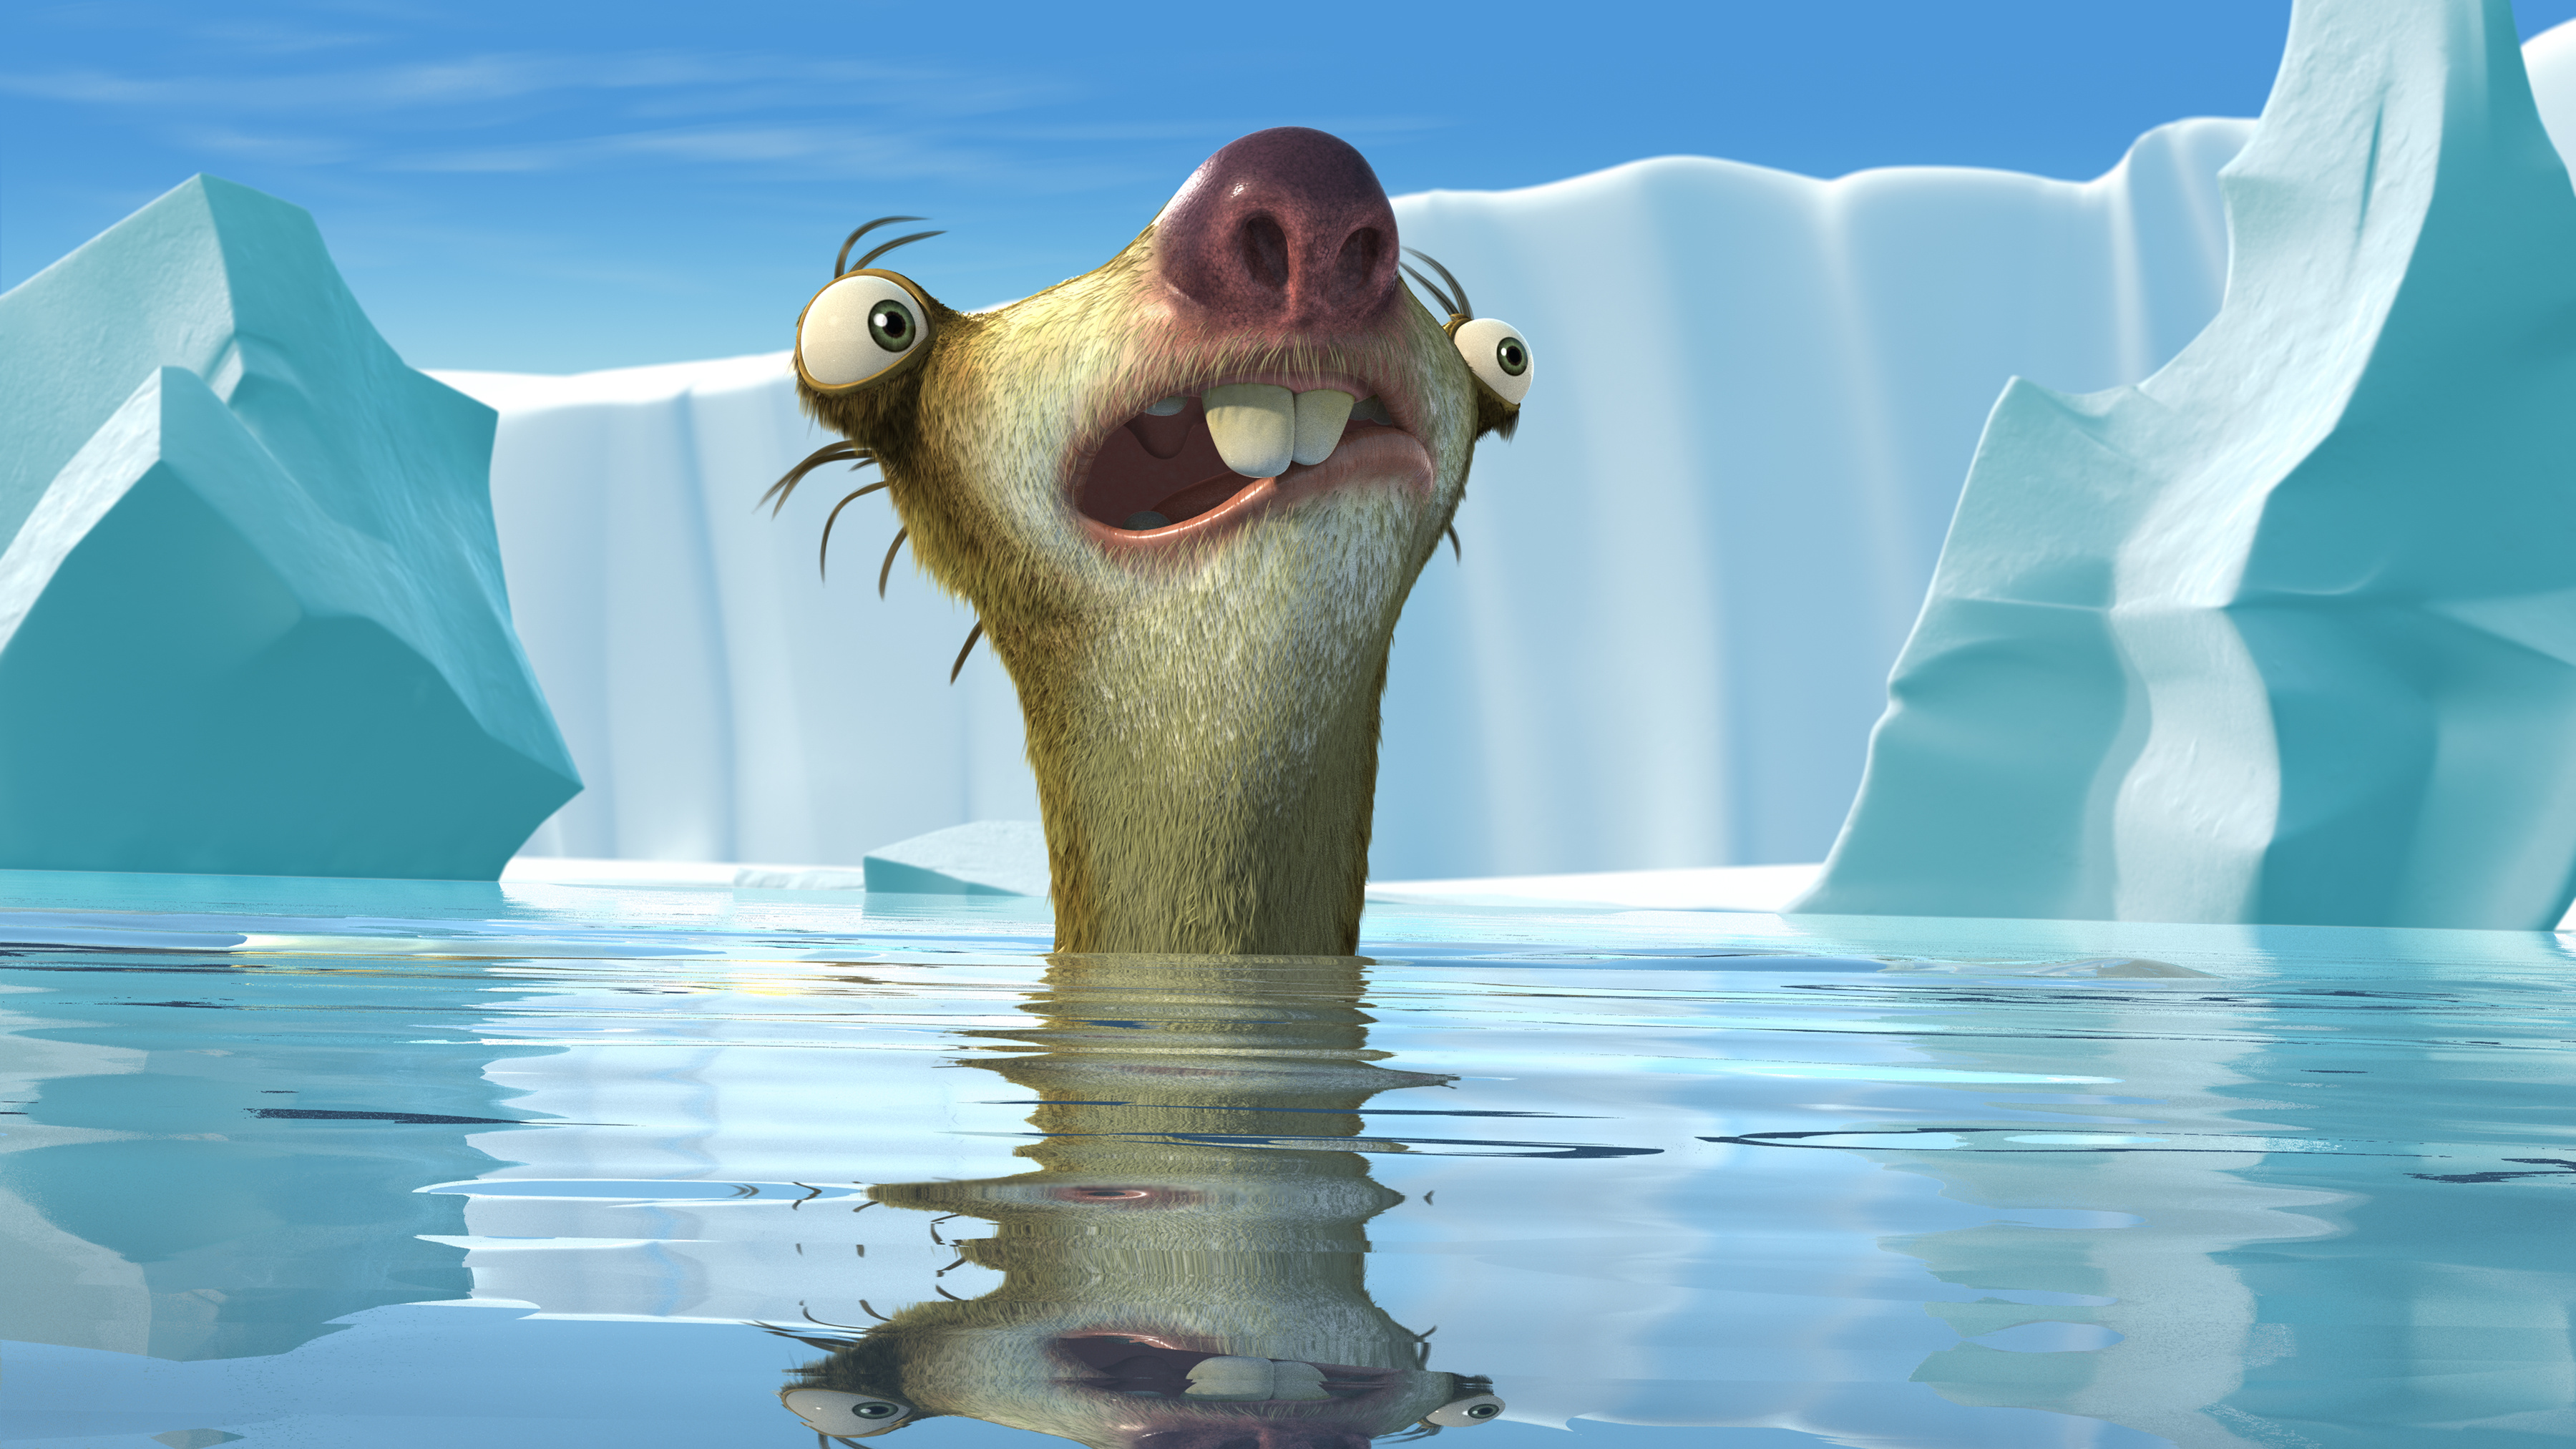
\includegraphics[height=\paperheight,width=\paperwidth]{ice-age}};}
}

\begin{frame}{Climate History}
  \vspace{.15cm}
  \begin{figure}
    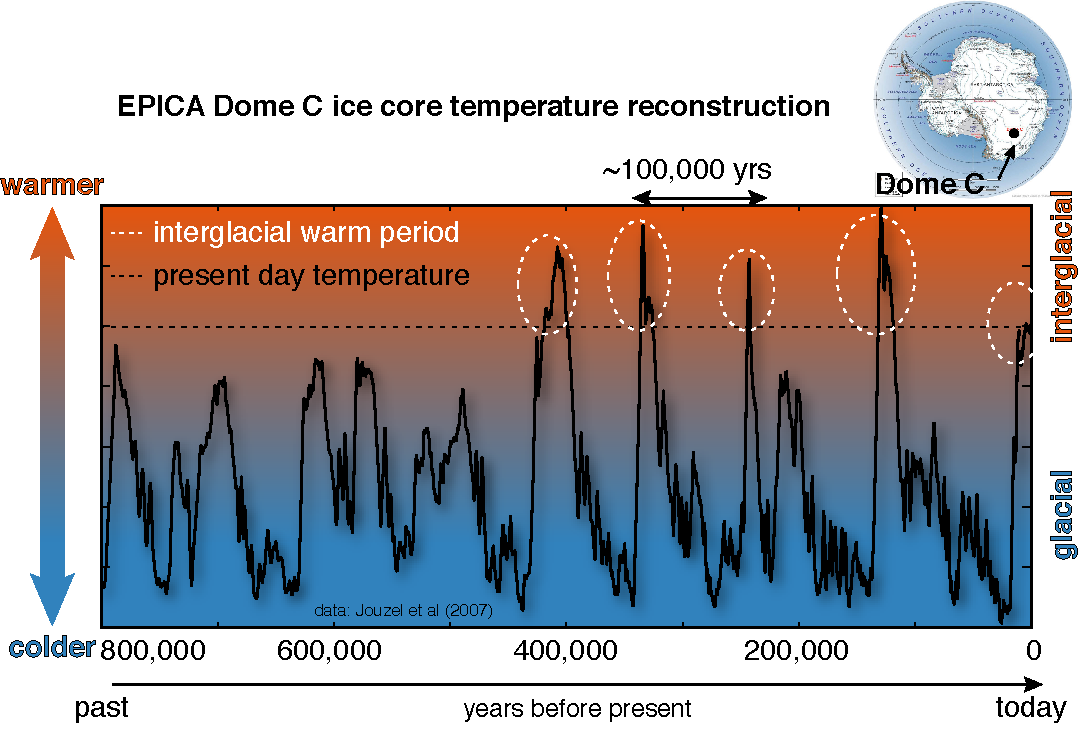
\includegraphics[width=\textwidth]{epica-temp}
  \end{figure}
  \note[item]{Let's look at temperature changes}
  \note[item]{What is this, explain time axis}
  \note[item]{We see that most of the time, it was cold and we were in an Ice Age}
  \note[item]{But find 5 distinct warm periods during the past half a million years, about 100,000 years apart}
  \note[item]{and we are currently in the fifth warm period or interglacial that started about 12,000yrs ago}
  \note[item]{There have been times when it was warmer than today}
  \note[item]{but the last time it was warmer was more the 100,000yrs ago }
  \note[item]{This cycle of glacials and interglacials is driven by how much sun light the Northern Hemisphere receives}
  \note[item]{The physics behind this is well understood but would take up a whole other talk}
\end{frame}


\setbeamertemplate{background canvas}
{
}

\begin{frame}{So what makes the past 100\,yrs so special}
  \begin{figure}
    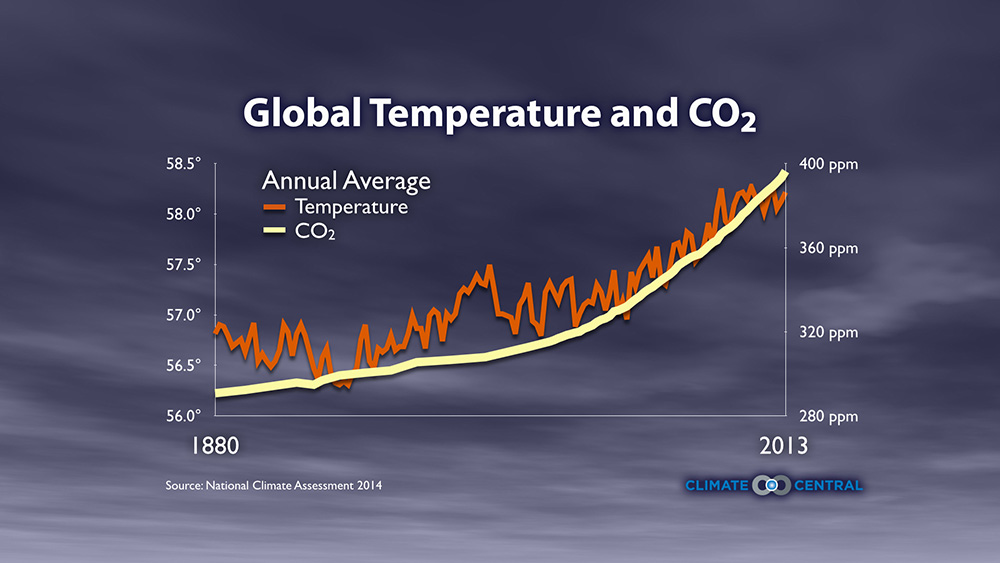
\includegraphics[width=\textwidth]{Global_Temp_and_CO2}
  \end{figure}
  \note[item]{Since I explained in the previous slide that whether we are in}
  \note[item]{an Ice Age or a warm period depends on how much sun we are receiving}
  \note[item]{one could suggest that increased sun is driving the current glacier mass loss}
  \note[item]{But if we look at sun activity, the sun activity has not increased considerably}
  \note[item]{so the sun is not the culprit, what else could it be?}
  \note[item]{Around the times of the Civil War, scientists discovered the Greenhouse effect}
  \note[item]{and by the end of the 19th century, we already knew that adding carbon dioxide to the atmosphere}
  \note[item]{will warm our planet}
  \note[item]{This relationship is illustrated in this figure here.}
  \note[item]{The orange curve shows temperature and the yellow curve shows CO2}
  \note[item]{And you can see that temperature follows CO2 quite well}
\end{frame}

  

\setbeamertemplate{background canvas}
  {
     \tikz{\node[inner sep=0pt,opacity=0.5] {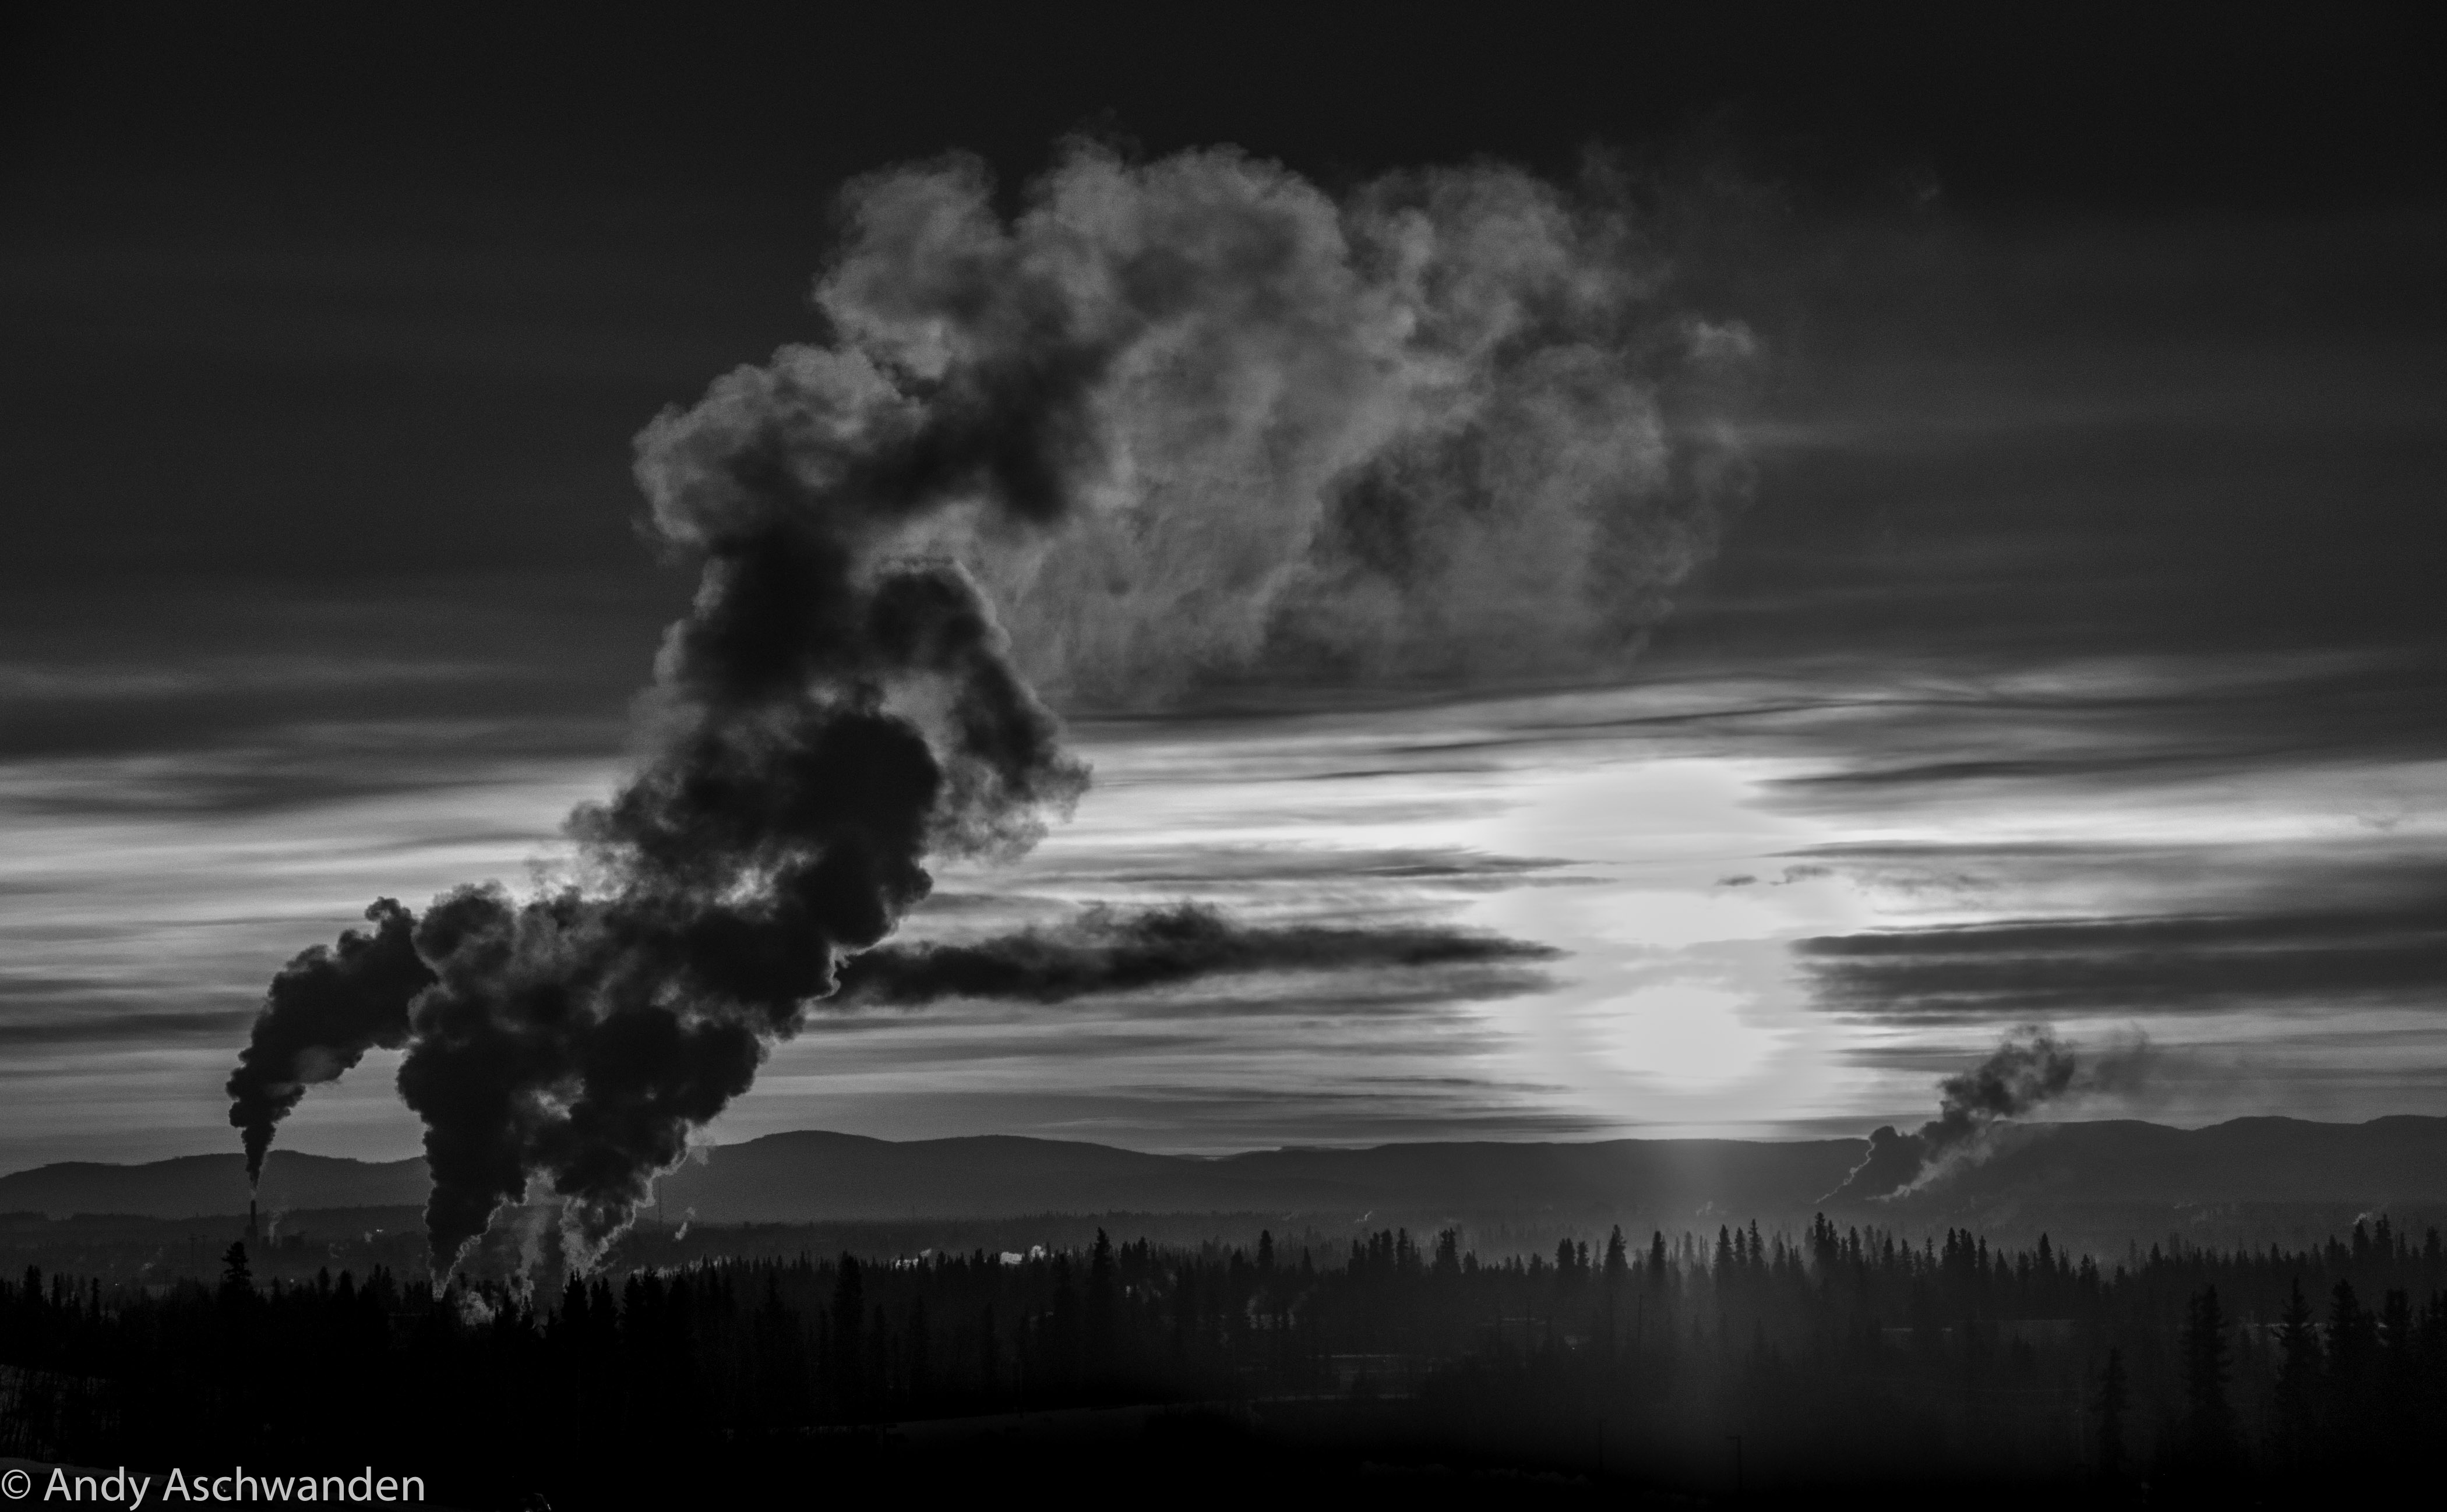
\includegraphics[height=\paperheight,width=\paperwidth]{uaf_power_plant}};}
} 

\begin{frame}{What if this trend continues?}
  \begin{itemize}
  \item Combustion of available fossil fuel resources sufficient to eliminate the Antarctic Ice Sheet (Winkelmann \emph{et al.}, 2015)
  \item and probably the  Greenland Ice Sheet too
  \item though this would take on the order of 10,000 years
  \end{itemize}
  \note[item]{Now that we know adding carbon dioxide to the atmosphere will make the world warmer}
  \note[item]{where does the additional carbon dioxide come from?}
  \note[item]{It mostly comes from us burning fossil fuels}
  \note[item]{where will this lead to?}
  \note[item]{My colleagues asked the a provocative question: what would happen if\ldots}
\end{frame}

\setbeamertemplate{background canvas}
  {
} 

\begin{frame}{What does this mean}
  \vspace{0cm}
  \begin{figure}
    \includegraphics<1>[height=0.9\textheight]{sea-level-potential-01}
    \includegraphics<2>[height=0.9\textheight]{sea-level-potential-liberty-01}
  \end{figure}
  \note[item]{How much ice can we melt?}
  \note<1>[item]{If all glaciers melted, Alaska, Switzerland, Himalaya, sea level would rise by 1 meter}
  \note<1>[item]{If the Greenland Ice Sheet melted, sea level would rise by 6 meter (or 20ft)}
  \note<1>[item]{If Antartica melted, sea level would rise by 60 meter (or 200ft)}
\end{frame}

\setbeamertemplate{background canvas}
  {
     \tikz{\node[inner sep=0pt,opacity=1] {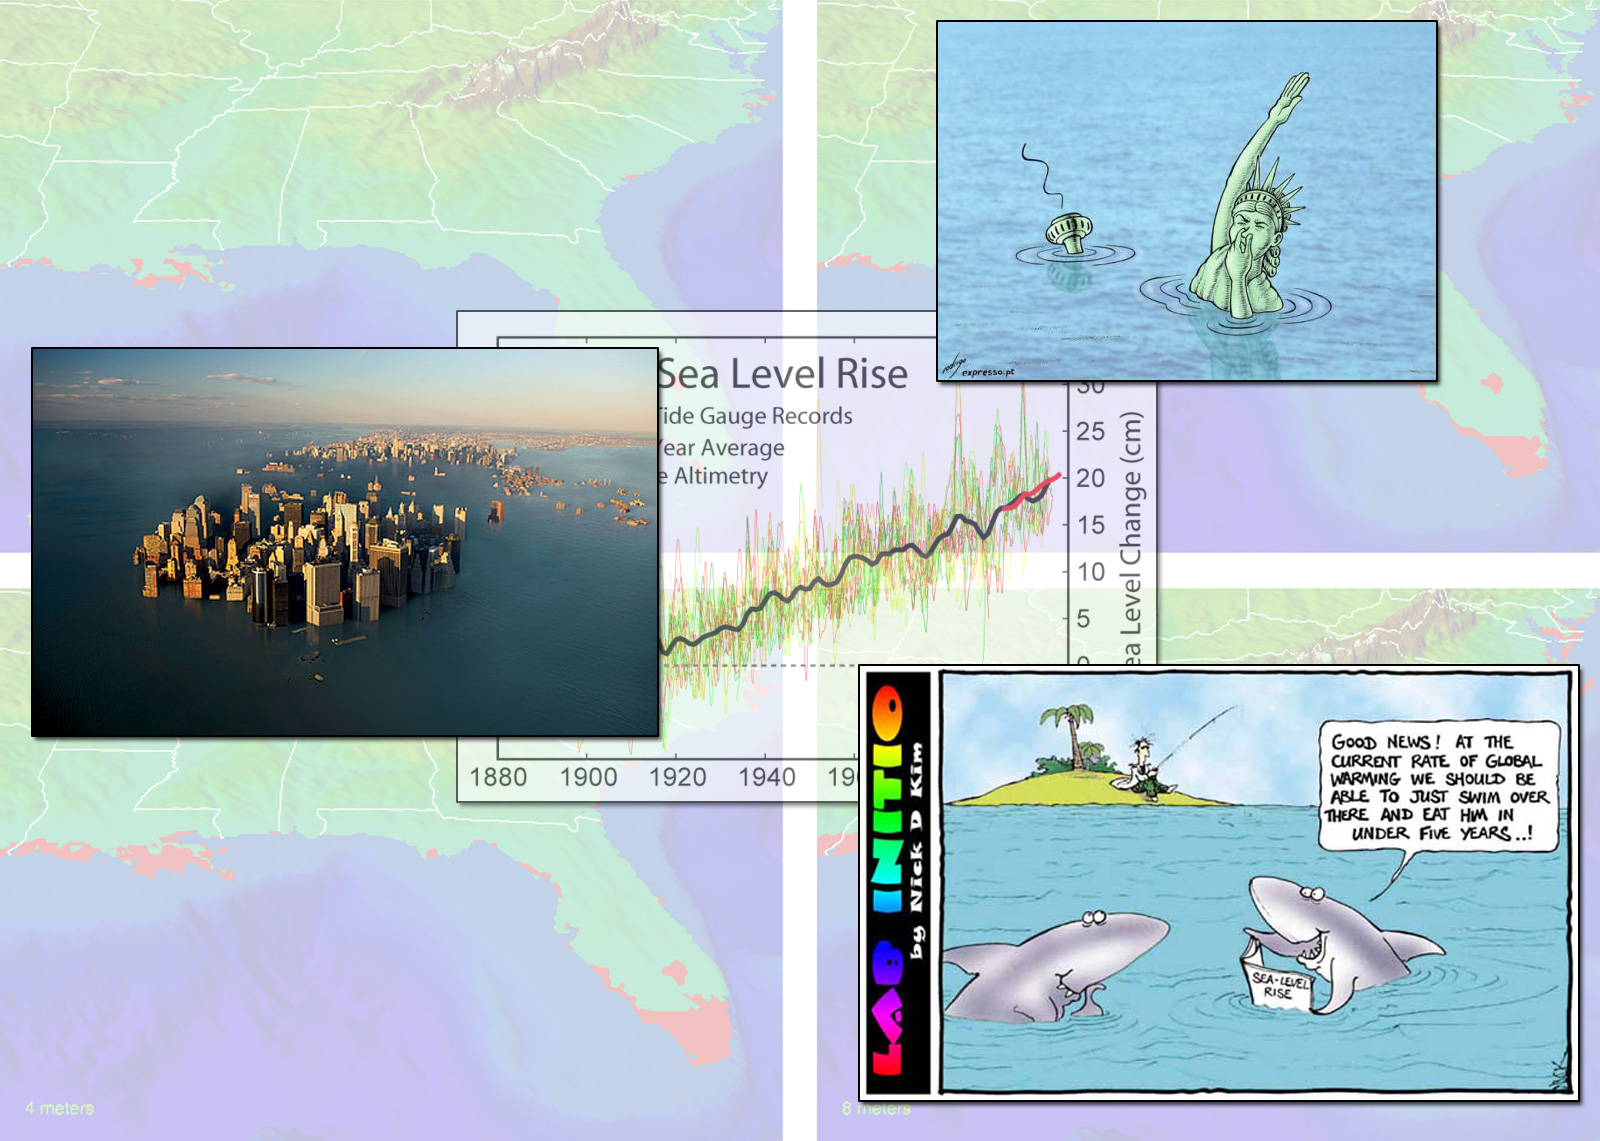
\includegraphics[height=\paperheight,width=\paperwidth]{sea_level_rise_composite}};}
} 

\begin{frame}{How realistic is all this?}
  \note[item]{What can we expect in the next century?}
  \note[item]{In recent years climate scientists and glaciologists}
  \note[item]{have gained a pretty good understanding of what rising air temperatures will}
  \note[item]{will do to our glaciers and ice sheets}
  \note[item]{but there is one aspect we have not yet talked about}
  \note[item]{and this is the role of the ocean}
  \note[item]{so in the remainder of the time, I would like to take you to a journey to Antartica}
\end{frame}


\setbeamertemplate{background canvas}
  {
     \tikz{\node[inner sep=0pt,opacity=1] {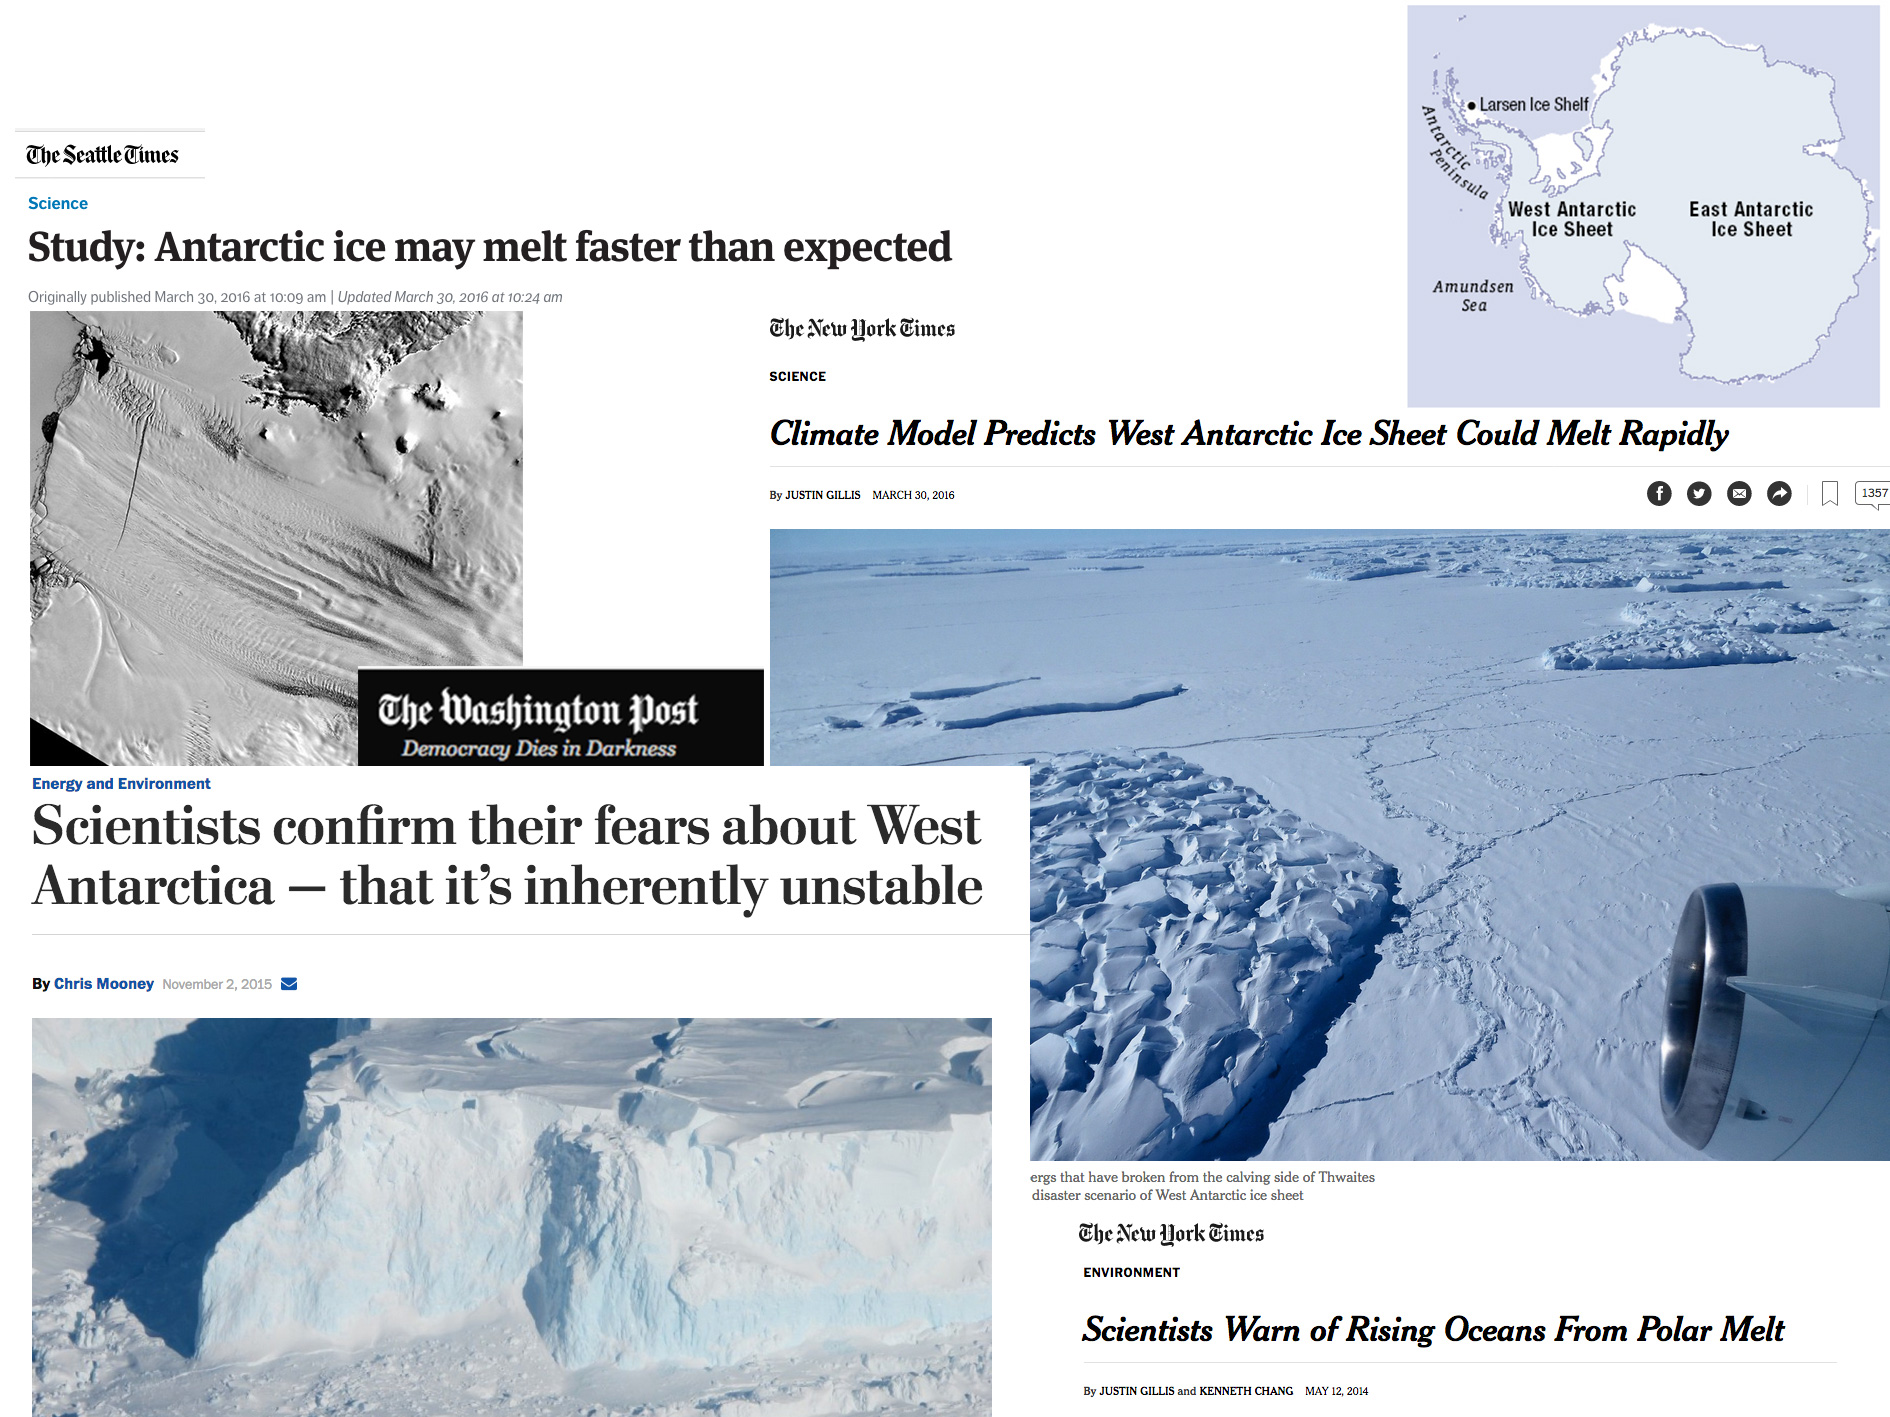
\includegraphics[height=\paperheight,width=\paperwidth]{wais-news}};}
} 

\begin{frame}{Antartica in the News}
  \note[item]{In the past 2--3 years, Antartica in general, and West Antartica in particular, has been in the news frequently}
  \note[item]{sometimes with rather scary headlines}
  \note[item]{why is there such a focus on Antartic research}
\end{frame}

\setbeamertemplate{background canvas}
  {
} 

\begin{frame}{Antartica The Continent}
  \begin{figure}
    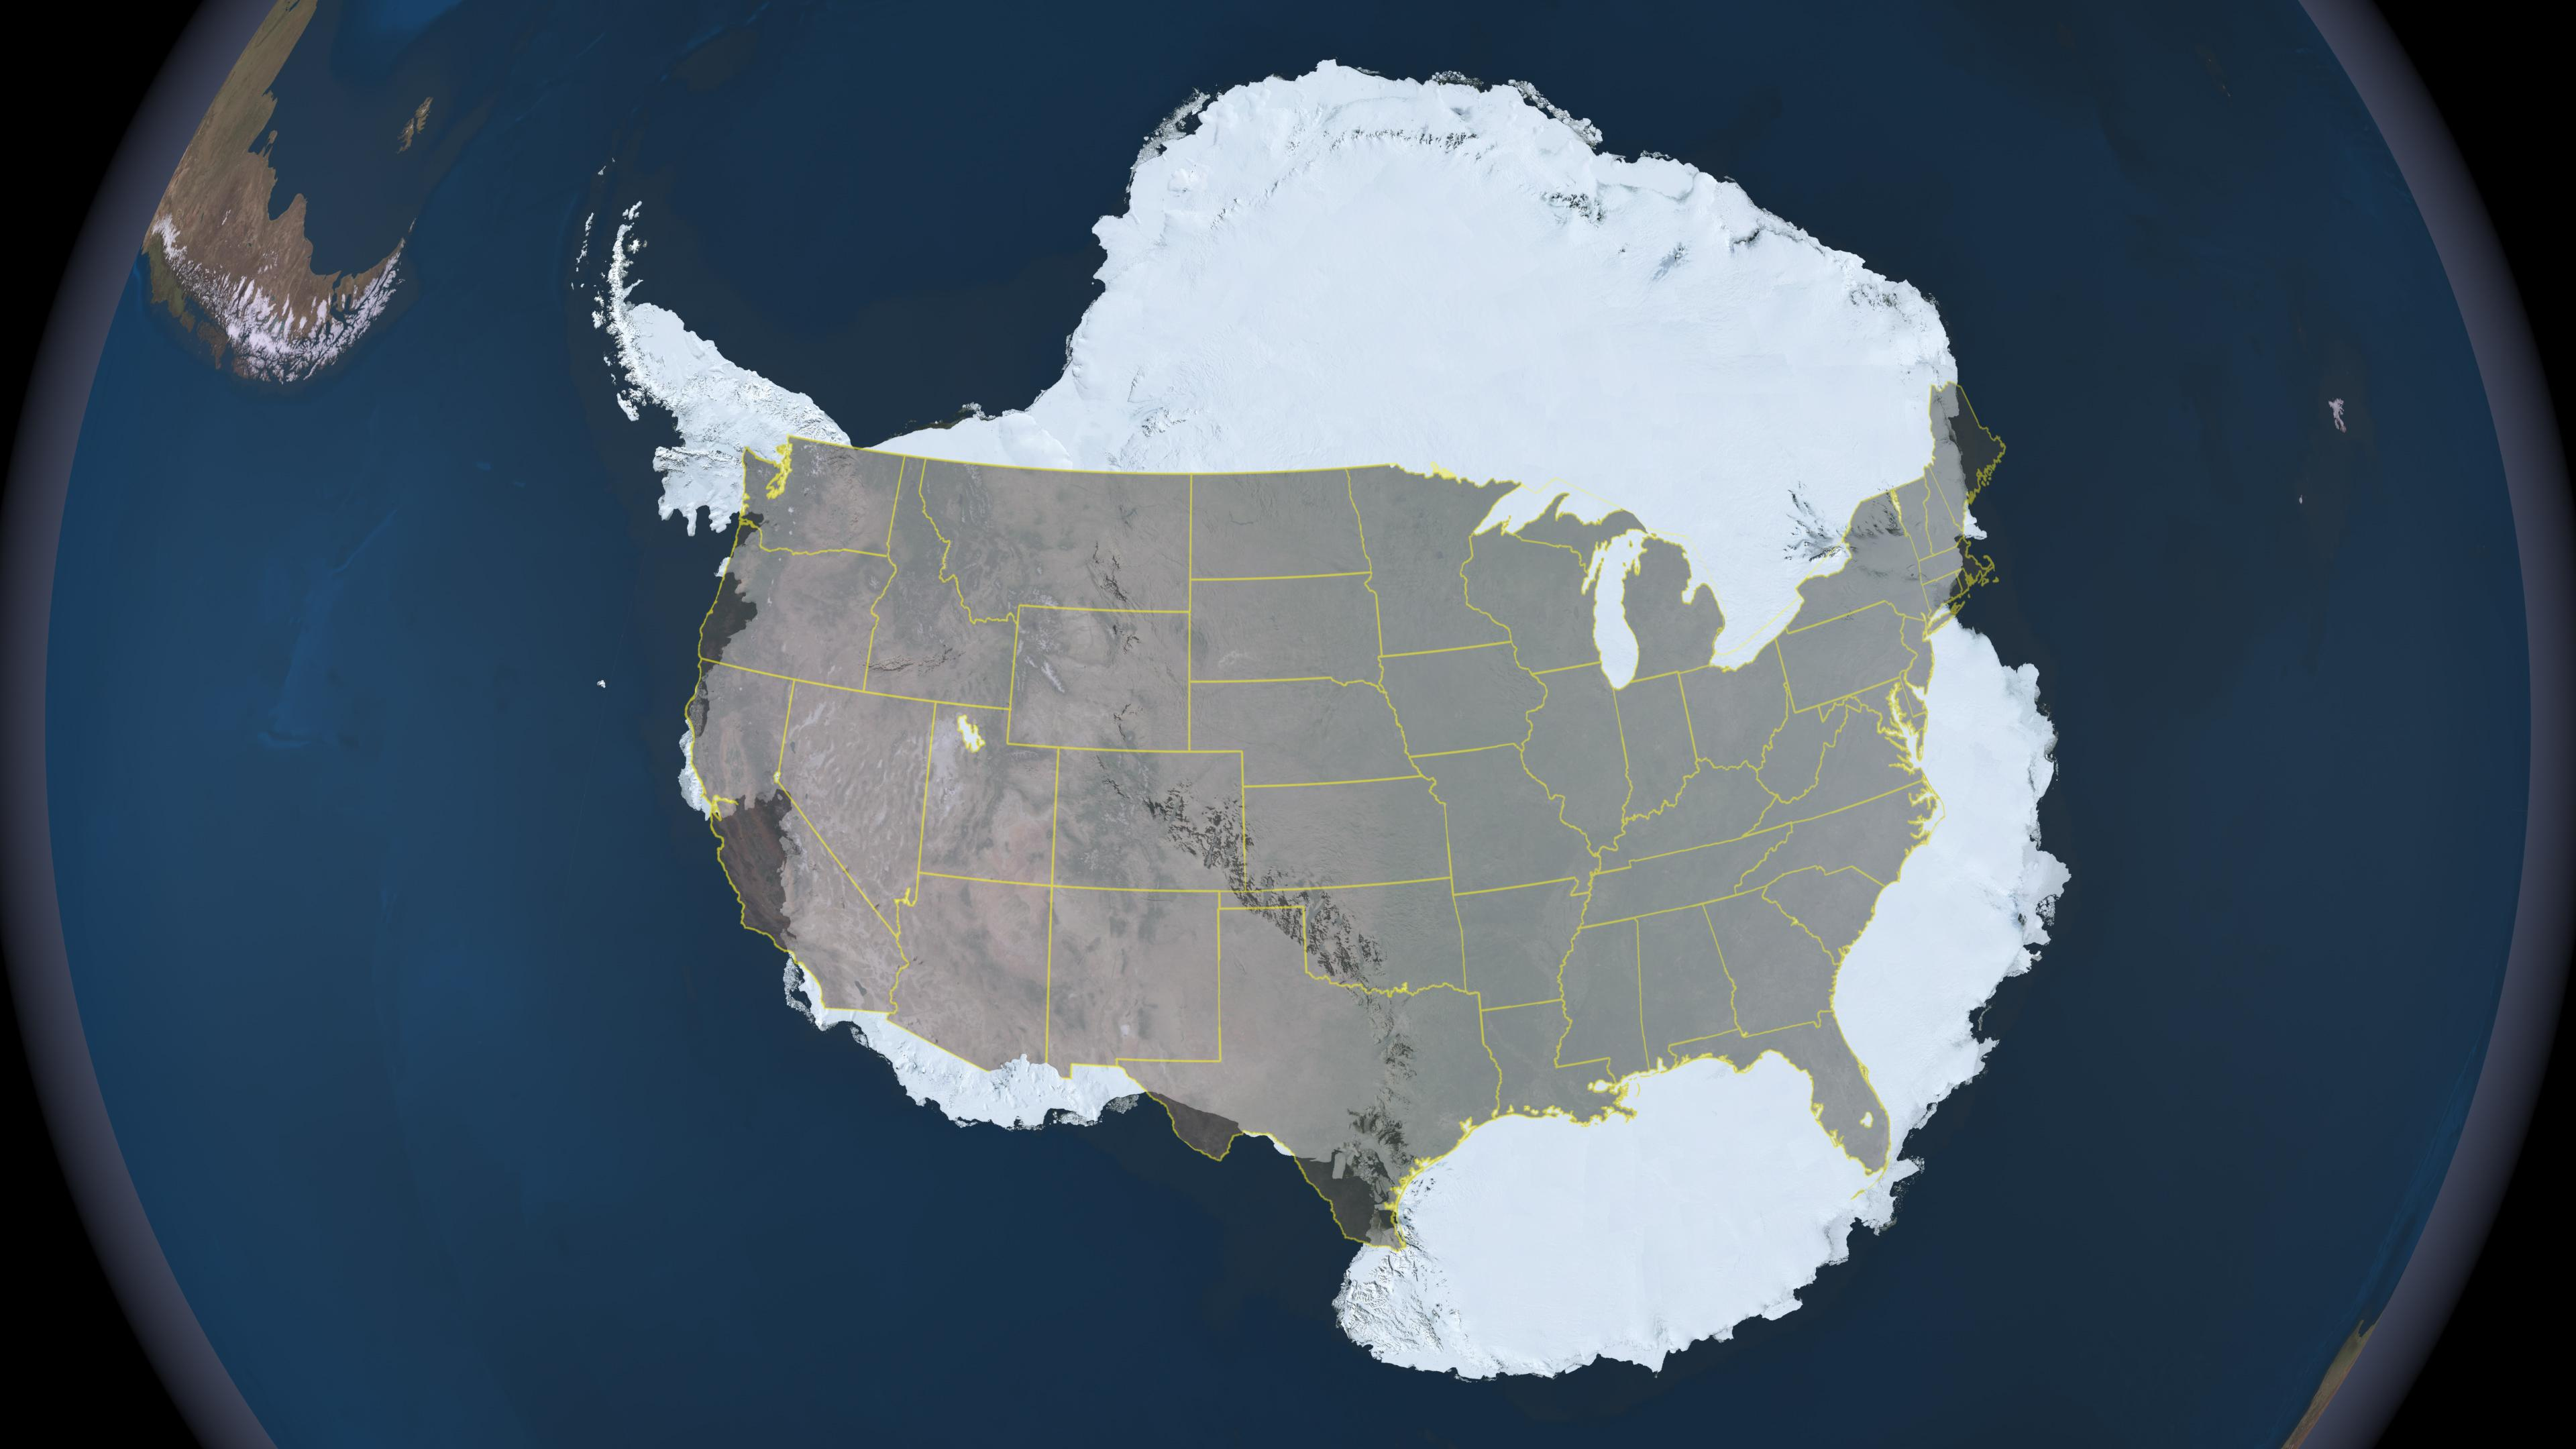
\includegraphics[width=\paperwidth]{main_USA_Antarctica_size}
  \end{figure}
  \note[item]{Antarctica is the highest, driest, coldest, windiest and brightest of the seven continents.}
  \note[item]{It is roughly the size of the United States and Mexico combined}
  \note[item]{and is almost completely covered by a layer of ice that averages more than one mile in thickness}
  \note[item]{but is nearly three miles thick in places.} 
  \note[item]{The ice sheet has been there for about 30 million years} 
\end{frame}


\setbeamertemplate{background canvas}
{
} 


\begin{frame}{The Antarctic Ice Sheet}
  \begin{figure}
    \includegraphics<1>[width=\textwidth]{ice-sheet-cartoon-simple}
  \end{figure}
  \note[item]{Antartica is a big blob of ice}
  \note[item]{Snow falls in the high interior and turns into ice}
  \note[item]{then the ice flows under its own weight to the coast}
  \note[item]{when it reaches the ocean, it becomes a float}
  \note[item]{and build up an ice shelf}
  \note[item]{then, from time to time, ice bergs break off of the shelf}
  \note[item]{there are two big difference between ice on land and shelf ice:}
  \note[item]{one is friction}
\end{frame}



\begin{frame}
  \begin{figure}
    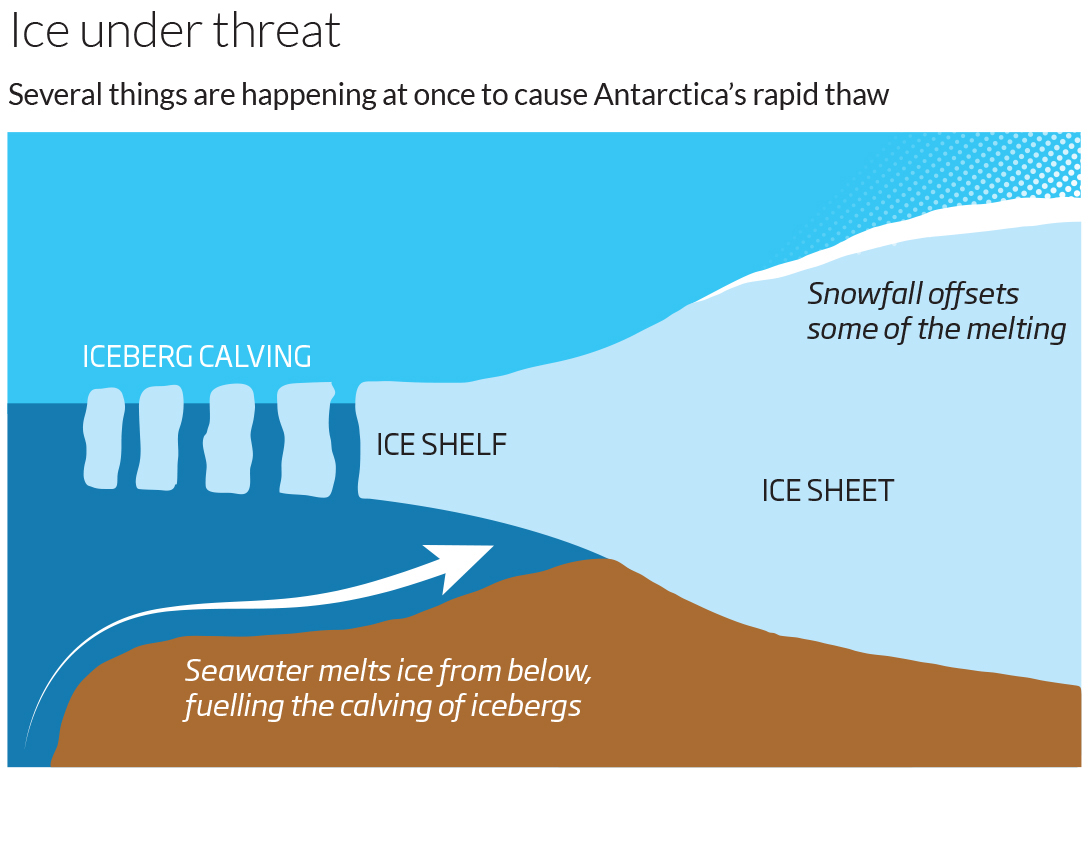
\includegraphics[width=\textwidth]{shelf-cartoon}
  \end{figure}
  \note[item]{the other difference is that}
  \note[item]{an ice shelf can be attacked from underneath}
  \note[item]{water is about four times more effective to melt ice than air}
  \note[item]{you can take it out of the freezer and put it on the counter}
  \note[item]{and wait. and wait. and wait.}
  \note[item]{at some point you'll be too hungry and you decide to cook something else}
  \note[item]{or you put the meat in a warm water bath, assuming it's vacuum sealed}
  \note[item]{and that's what is happening in Antarctica}
  \note[item]{the oceans are getting warmer and deliver more heat and melt more ice}
\end{frame}


\begin{frame}{Attack from below}
 \begin{figure}
  \movie[showcontrols=true,autostart,loop,width=10cm]{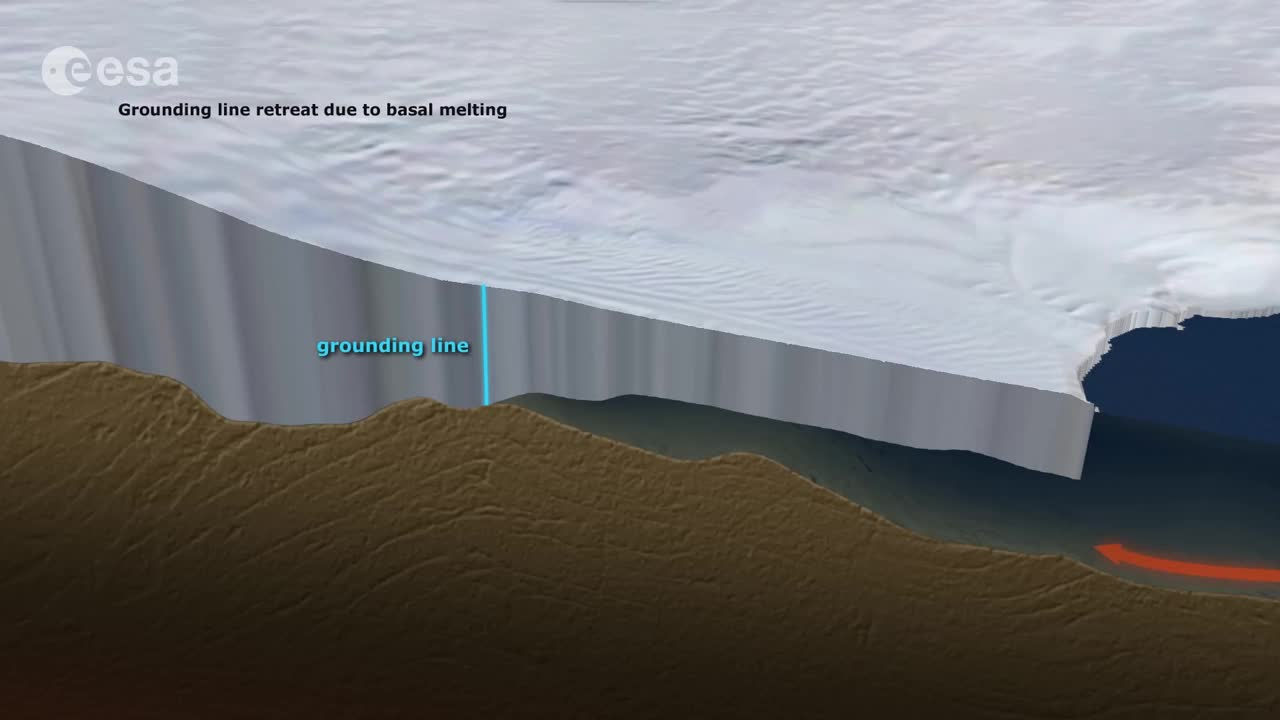
\includegraphics[width=10cm]{gl-retreat}}{gl-retreat.mov}
  \end{figure}
  \note[item]{Here you see an animation of the process}
  \note[item]{In the beginning, the shelf is thick and healthy}
  \note[item]{but warm water is on its way to attack the shelf}
  \note[item]{the shelf thins and retreats}
  \note[item]{at some point the shelf will become so thin that it will break off}
  \note[item]{and that's what we are so concerned about}
\end{frame}

\begin{frame}{Antarctica's Ice Shelves}
  \begin{figure}
    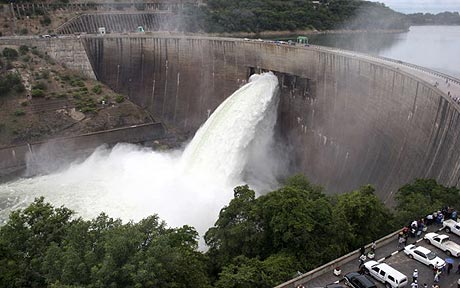
\includegraphics[height=5cm]{dam-breaking}
  \end{figure}
  \note[item]{ice shelfs as like a plug or a flood gate}
  \note[item]{it hold the interior ice back}
  \note[item]{once the plug is removed or the gate is open}
  \note[item]{there is nothing holding the ice behind it back}
\end{frame}


\begin{frame}{Antarctica's Ice Shelves}
  \begin{figure}
    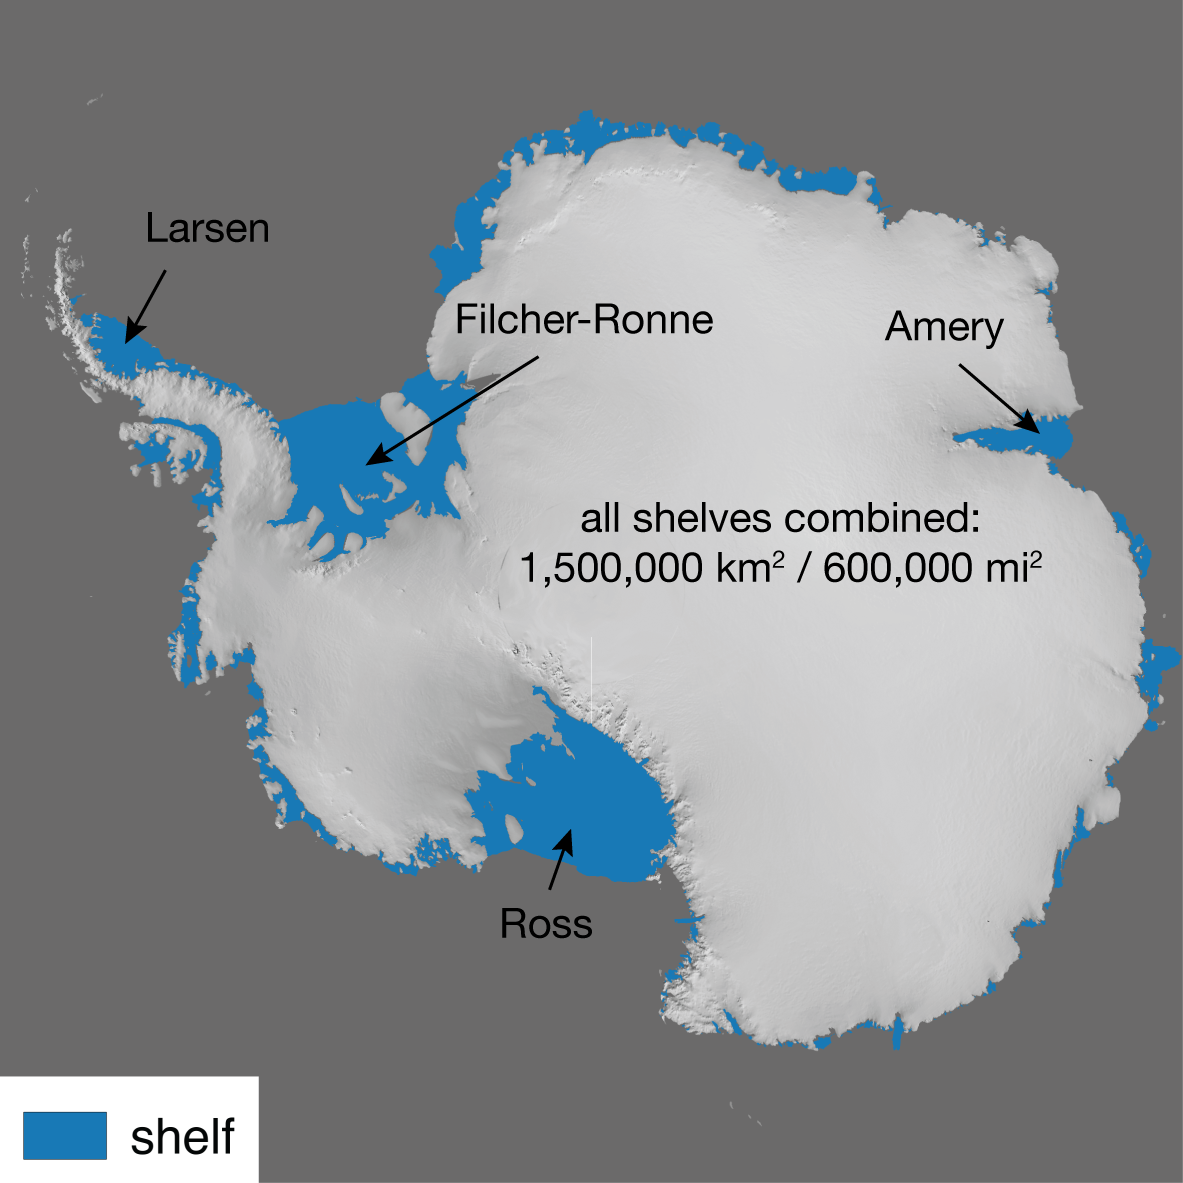
\includegraphics[height=0.9\textheight]{ant-ice-shelves-map}
  \end{figure}
  \note[item]{Antartica is surrounded by ice shelves}
  \note[item]{Who knows the size of Alaska?}
  \note[item]{There is a lot at stake here}
  \note[item]{There is a particular area in West Antartica called the Amundsen Sea Embayment}
  \note[item]{where some think the retreat is already under way and unstoppable}
\end{frame}


\begin{frame}{West Antarctic Ice Sheet}
  \movie[showcontrols=true,width=10cm]{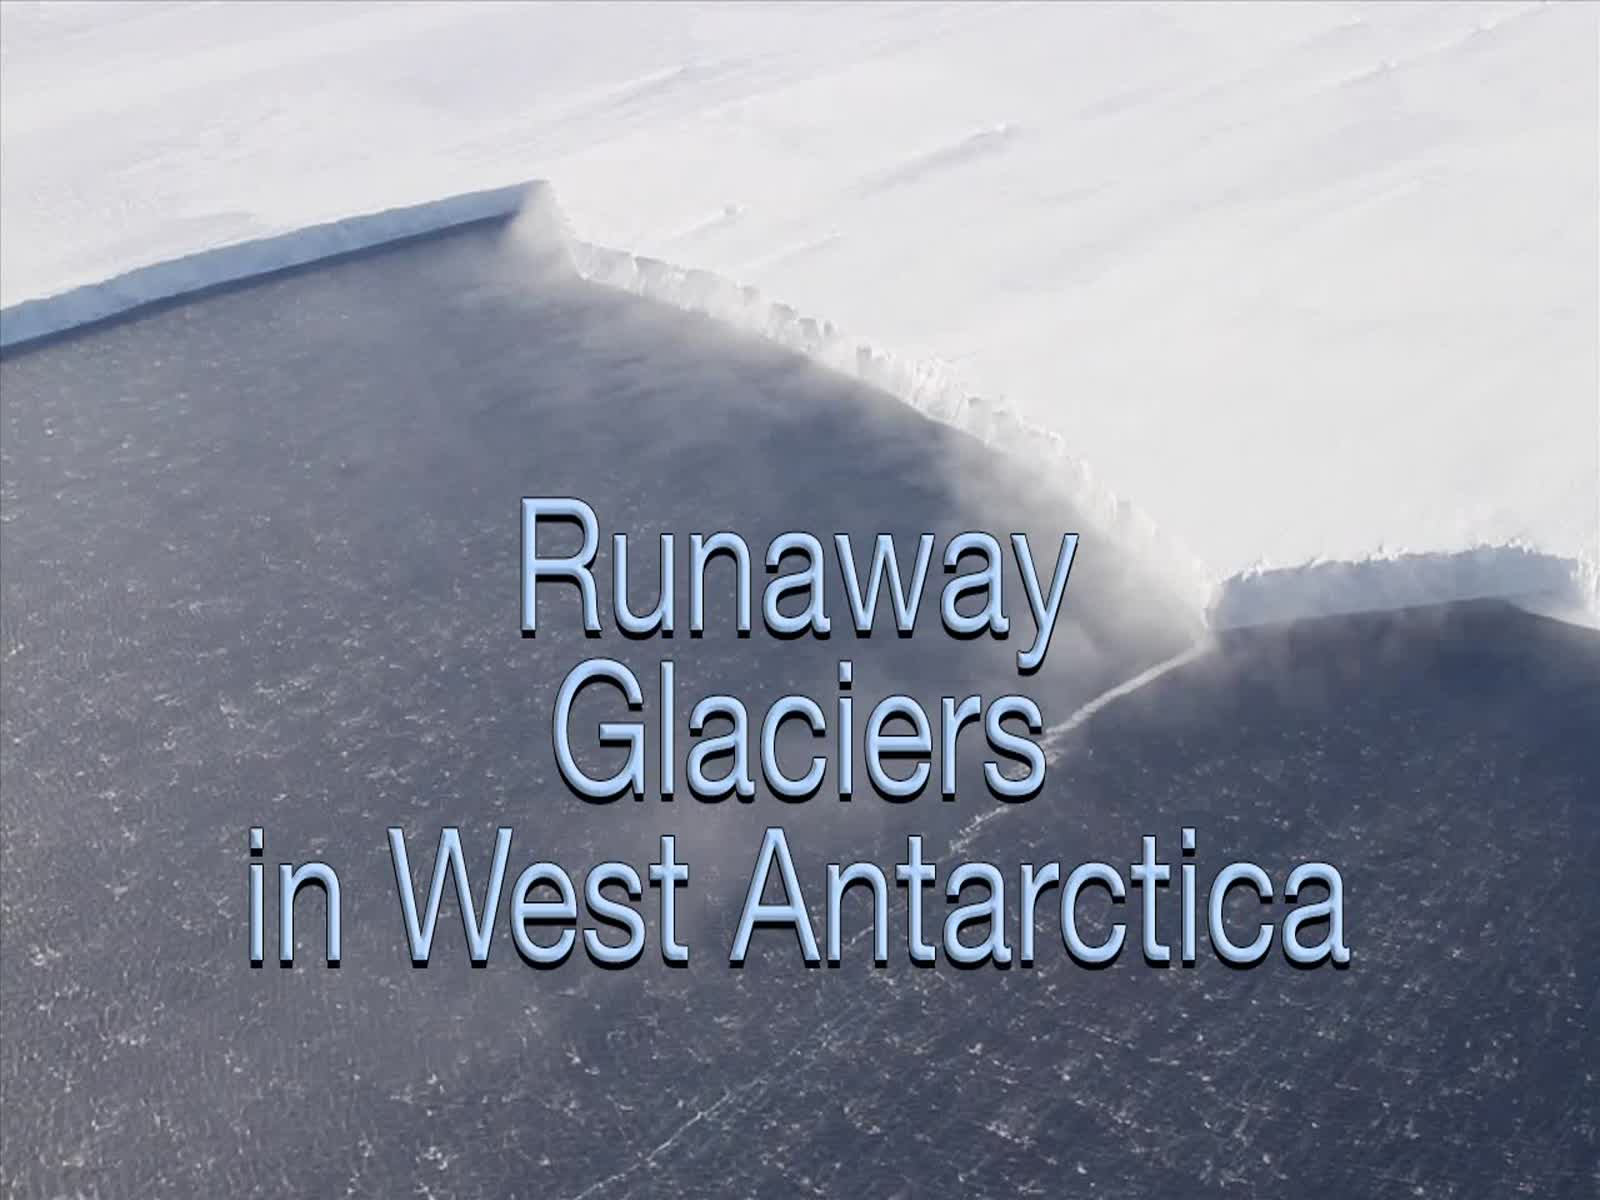
\includegraphics[width=10cm]{rignot-wais}}{rignot-wais.mov}
  \note[item]{Here is my colleague Eric Rignot}
\end{frame}

\begin{frame}{Going Forward}
  \begin{figure}
    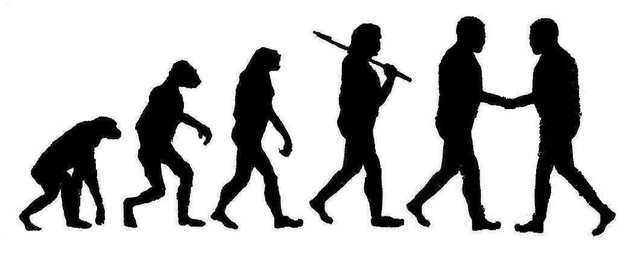
\includegraphics[width=\textwidth]{adaptation}
  \end{figure}
\note[item]{How much of West Antartica is going to melt is still an active topic of research}
\note[item]{our latest model simulations show 20\,cm--1\,m by 2100 from Antarctica}
\note[item]{this may sound very scary}
\note[item]{but I would like to end with a positive thought:}
\note[item]{Between the last glacial maximum 20,000yrs ago and today}
\note[item]{sea level has risen by 100\,m during a time when humans were around}
\note[item]{this shows that}
\note[item]{if we all work together, we will be able to adapt to these changes}
\end{frame}



\setbeamertemplate{background canvas}
{
  \tikz{\node[inner sep=0pt,opacity=1] {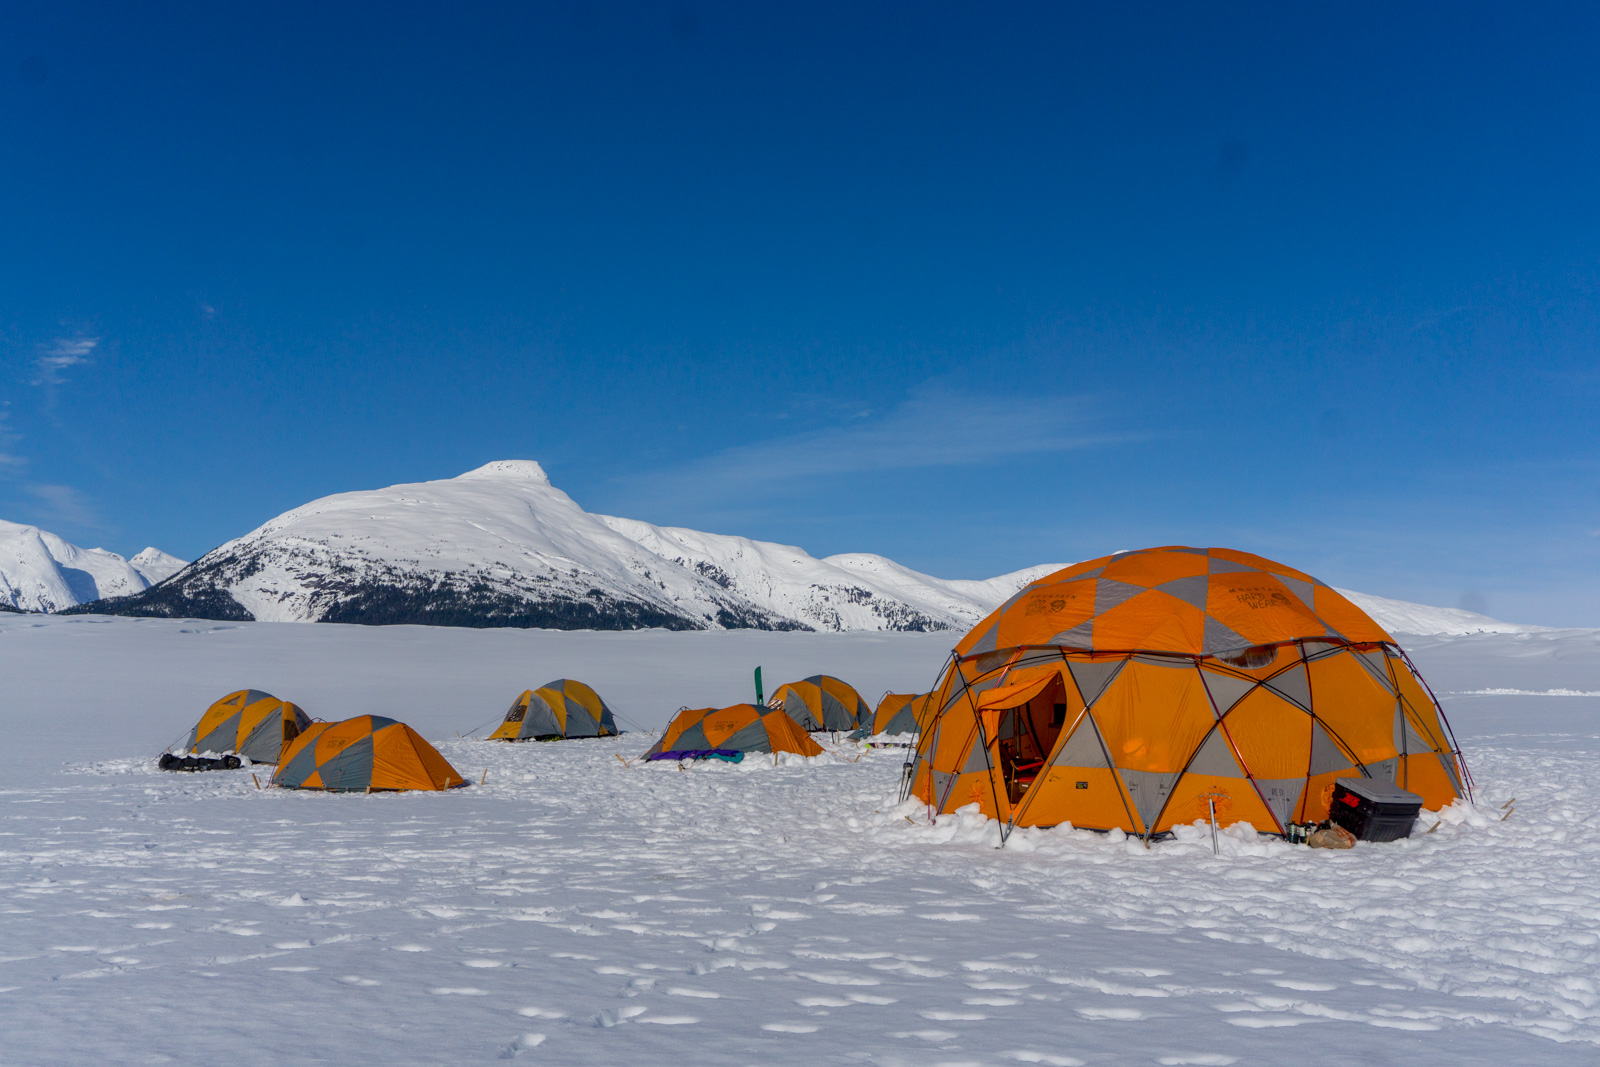
\includegraphics[height=\paperheight,width=\paperwidth]{taku-8}};}
}

\begin{frame}{Questions?}

\end{frame}

\setbeamertemplate{background canvas}
{
}

\begin{frame}{The sun drives the glacial/interglacial cycle}
  \vspace{-2cm}
  \begin{block}{Milankovitch Cycle}
    \begin{figure}
      \movie[showcontrols=true,autostart,loop,width=8cm]{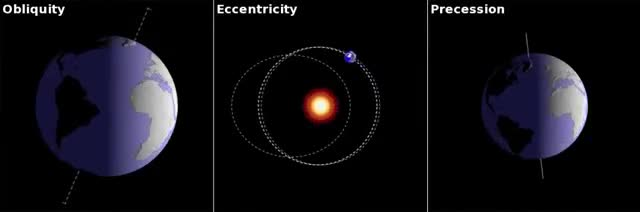
\includegraphics[width=8cm]{orbital-forcing}}{orbital-forcing.mov}
    \end{figure}
  \end{block}
  \begin{columns}[T]
    \begin{column}{.32\linewidth}
      41,000 yrs
    \end{column}
    \begin{column}{.32\linewidth}
      100,000 yrs
    \end{column}
    \begin{column}{.32\linewidth}
      26,000 yrs
    \end{column}
  \end{columns}
  \note[item]{Changes in the obliquity (tilt) of Earth's axis}
  \note[item]{Variations in the shape of Earth's orbit (eccentricity)}
  \note[item]{Changes in Earth's "Wobble" (Precession)}
  \note[item]{ When less solar energy is received earth enters into an ice age; when earth begins to receive more solar energy it comes out of the ice age. The amount of solar energy and the resulting changes to temperature this has can be worked out and it amounts to around 5 degrees C.}
  \note[item]{The additional rise and fall in temperatures beyond the 5 degrees C range can only be explained by the effects of CO2 concentration in the atmosphere due to various feedback or forcing mechanisms.}
  \note[item]{As the earth's temperature begins to drop feedback occur that reduce the amount of CO2 being produced and atmospheric concentrations begin to fall.}
  \note[item]{At the end of an ice age as more solar energy is received and again as temperatures begin to rise; feedbacks begin to produce more CO2 increasing CO2 concentrations.}
\end{frame}


\begin{frame}
    \begin{figure}
      \movie[showcontrols=true,loop,width=10cm]{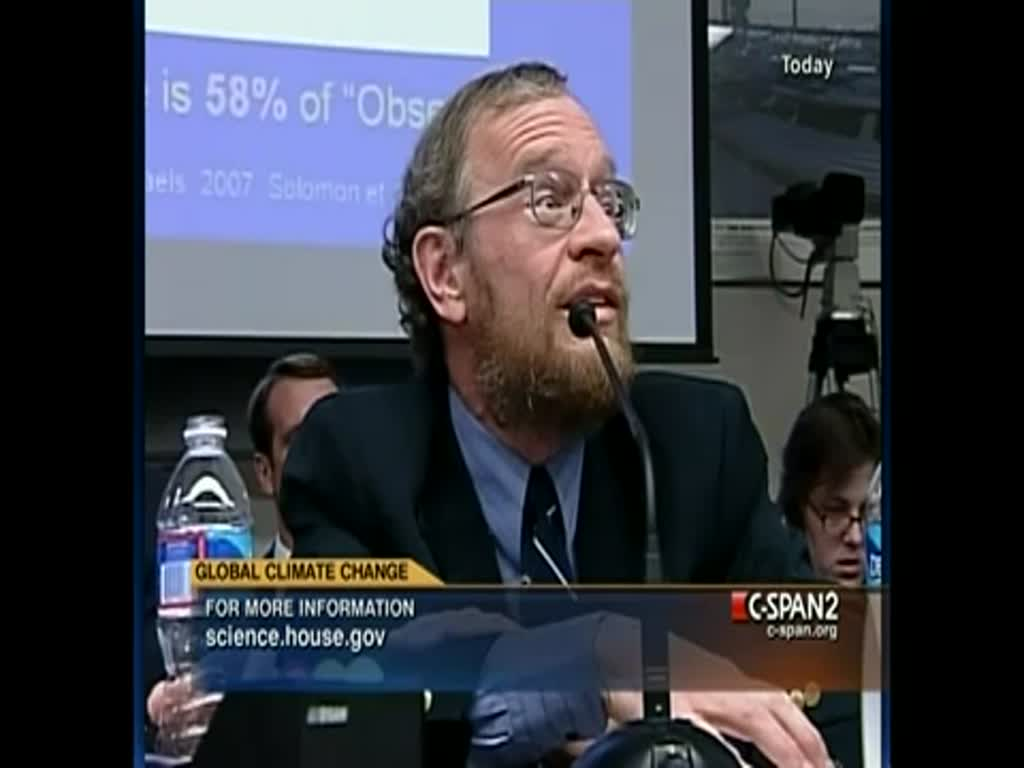
\includegraphics[width=10cm]{alley-001}}{alley-milankovitch.mov}
    \end{figure}
    \note[item]{My colleague Richard Alley is much more eqloquent in explain what causes ice ages}
    \note[item]{as he did in this hearing in front of congress a couple of years ago}
\end{frame}

\begin{frame}{The Greenhouse Effect\ldots{}is not rocket science}
  \begin{itemize}
  \item The existence of the greenhouse effect was argued for by Joseph Fourier in 1824.
  \item The argument and the evidence were further strengthened by Claude Pouillet in 1827 and 1838 
  \item and reasoned from experimental observations by John Tyndall in 1859, who measured the radiative properties of specific greenhouse gases.
  \item The effect was more fully quantified by Svante Arrhenius in 1896, who made the first quantitative prediction of global warming due to a hypothetical doubling of atmospheric carbon dioxide
  \end{itemize}
\end{frame}

\begin{frame}{Carbon Dioxide}
      \begin{figure}
        \includegraphics<1>[width=\textwidth]{nasa_co2-graph}
      \end{figure}
\end{frame}


\end{document}

